\chapter{Learning to identify clause types in English}
\label{chap:eng-cl}


As discussed in the previous chapters, cross-linguistically we see three major clause types, declaratives, interrogatives, and imperatives, corresponding to three main speech acts, assertions, questions, and commands/requests. We also saw in Chapter~\ref{chap:background} that by 18 months old, infants seem to have figured out clause types and their canonical functions, i.e., the type of speech acts they are canonically used for.  As discussed in Chapter~\ref{chap:introduction}, the acquisition of clause types can be decomposed into two challenges: 1) the clustering problem, i.e. clustering clauses in the right three categories, and 2) the \tbf{labeling problem}, i.e. linking each category to its function. 

%Given that infants's early success at identifying clause types,
This chapter investigates how learners solve these problems, especially the clustering problem, by probing the extent to which children need to rely on pragmatic information (i.e., inferring what speech act a given utterance of sentence is conveying). As discussed in Chapter~\ref{chap:introduction}, pragmatic information is essential for solving the labeling problem. The question I ask here, then, is whether pragmatic information is also crucial for solving the clustering problem, or, conversely, if it might hurt. Will a learner strictly tracking formal regularities home in on the right three clusters of clauses? Will a learner privy to some speech act information fare better? Does the speech act information help or hurt the learner? It can help by highlighting which formal distinctions matter for clause typing; it could hurt if clause types are systematically used in indirect speech acts. If pragmatic information like speech act helps, how much pragmatic information is required? 

To answer these questions, I compare the performance of two computational models, a \gls{dlearnerabbr} and a \gls{plearnerabbr}. Since the success of the learning models should be commensurate with infants' early successes at identifying clause types, I test the models using data from an annotated dataset created with parental sentences in the Providence Corpus (\cite{ProvidenceCorpus}). I will show that the \gls{dlearnerabbr} fail to identify all three clause types, suggesting that the morpho-syntactic information alone is not sufficient for learning clause types, and pragmatic information, i.e. the speech act that a sentence is used to perform, is crucial.

But how much pragmatics is needed, I manipulate the ratio of noise in the pragmatic information. I will show that learners need very little pragmatic information to help them figure out clause type. Even with 80\% noise, models with speech act information still outperform the one without.

In this chapter, I assume that learners can have access to pragmatic information. Chapter~\ref{chap:eng-sp} will address the question of how learners might be able to glean speech act information other than relying on clause types. 

This rest of the chapter is organized as follows: 
In Section~\ref{sec:engcl:background}, I first briefly introduce the two computational models mentioned above, and how they can help us answer our questions (Section~\ref{sec:engcl:bg:learners}). I then review the formal features of English \diis{} (Section~\ref{sec:engcl:bg:grammar}), setting the stage for discussing the learning of these clause types. But these are features that English employs for clause typing, infants at 18 months old might not be able to perceive all of these features. To allow our models to best capture 18-month-olds' learning process, we need to look at 18-month-olds' linguistic capacity and knowledge with regard to these features. So in Section~\ref{sec:engcl:bg:assumptions} I briefly go through the linguistic capacities and knowledge of infants before 18 months old with regard to the formal features used for clause typing, which in turn will guide the way these features are coded in the corpus. 

In Section~\ref{sec:engcl:corpus}, I report results from a corpus study on parents' use of different clause types and speech acts, to give a quantitative description of the information present in the input. The annotated dataset that results from this corpus study will be used in our modeling experiments.

Section~\ref{sec:engcl:model} details the two computational models for the two learners, \gls{dlearnerabbr} and \gls{plearnerabbr}, to see if pragmatic information is needed for solving the clustering problem. I then manipulate the ratio of noise in the pragmatic information to see how much pragmatics is needed (Section~\ref{sec:engcl:model:noisy}). \revise{One feature not addressed in chapter is prosody. As we have discussed in Chapter~\ref{chap:background}, the role of prosody might be complicated. We will turn to prosodic features in Chapter~\ref{chap:prosody}.}

\section{Background}
\label{sec:engcl:background}

\subsection{Two learners} 
\label{sec:engcl:bg:learners}
As mentioned above, the question we set out to answer is whether morpho-syntactic features alone are sufficient for learners to solve the clustering problem. To this end, I build two computational models that learn the clustering of clauses, a \text{\distlearner{}} (\dlearnerabbr{}) and a \text{\praglearner{}} (\plearnerabbr{}). Both learners are forms of distributional learning: they track distributions of certain features in their input, and use these observations to infer the underlying categories that gives rise these distributions
(cf. \cite{feldman2013,gagliardi2017modeling,perkins2022vmodel,perkins2019,nguyenwilson2021}; see \cite{pearl2020review} for a recent review). Specifically, these two learners share the same goal of discovering the underlying clustering of sentences in parents' speech, i.e. to infer the abstract clause type categories in English. The difference between them lie in the sources of information they take as input. 

The \tbf{\distlearner{}} (\dlearnerabbr{}) assumes that learners track the statistical distributions of \tit{morpho-syntactic features} present in the surface forms of sentences to infer the abstract clause type category that gives rise to these distributions. This learner serves as our baseline; by looking at its performance, we will be able to see whether syntactic information by itself is sufficient for identifying clause types. 

The \tbf{\praglearner{}} (\plearnerabbr{}) also tracks the distributions of morpho-syntactic features, but at the same time, it keeps track of the speech acts expressed by these sentences as well. Thus, it infers clause type categories with information from both syntax and pragmatics. 

Thus, we would be able to answer the question of whether pragmatics is crucial for the clustering problem by comparing the performance of these two learners: if pragmatic information helps the learner, not only with labeling but also with clustering, we would see \plearnerabbr{} outperforms \dlearnerabbr. Additionally, if \plearnerabbr{} performs better, we can manipulate the ratio of noise in the pragmatic information that \plearnerabbr{} receives, to see how much pragmatic is needed for learners to solve the clustering problem. 


The success of these two learners depend on the specific features we feed into the models. In Chapter~\ref{chap:background}, we reviewed different taxonomies for speech act information and we may abstract away from language-specific ways of indicating force by having the \plearnerabbr{} keep track of pragmatic information in terms of knowing whether a sentence is an assertion, question or request. But the morpho-syntactic features for clause typing differ from language to language and to test whether the \dlearnerabbr{} can acquire clause typing from morphosyntax alone, we must test it on the actual features of the language we test it on. So, in the next section, we will go through the specific morpho-syntactic features that English employs for clause typing, to set the stage for our discussion of the learning of clause types. 


\subsection{Clause types in English} \label{sec:engcl:bg:grammar}

Generally, clauses in English are marked by the presence of verbs (\ref{ex:engcl:fragments}a). Sentences without verbs are often classified as fragments (\cite{sz1985speechact}), as in (\ref{ex:engcl:fragments}b):
\bex{ex:engcl:fragments}
\bxl{}
Mary hugged Ann.
\ex
Mary!
\exl
\eex

In this section, we will go over the properties of the three major types of clauses, \diis{}, in English. 
It is generally assumed that the declarative is the default clause type in English, and thus has the formal features [-int, -imp]. The hallmark of the [+int] value of English $C$ is subject-auxiliary inversion, which can be seen in polar interrogatives like  (\ref{ex:engcl:subjaux}a) and \twh-interrogatives like (\ref{ex:engcl:subjaux}b). 

\bex{ex:engcl:subjaux}
\bxl{}
Can Mary hug Ann?\hfill polar interrogative
\ex
Who can Mary hug? \hfill \twh-
interrogative
\exl
\eex


However, this association of word order and interrogativity has many exceptions. For example, in subject \twh-interrogative sentences like (\ref{ex:engcl:int-exceptions}a) and sentences with embedded interrogatives (\ref{ex:engcl:int-exceptions}b-c), the interrogative takes the same word order as a declarative. 

\bex{ex:engcl:int-exceptions}
\bxl{}
Who can hug Ann? \hfill subject \twh-interrogative
\ex
Mary wonders \tun{who Ann can hug.} \hfill embedded \twh-interrogative
\ex 
Mary wonders \tun{whether Ann can hug Sue.} \hfill embedded polar interrogative
\exl
\eex

As discussed in Chapter~\ref{chap:introduction}, these cases might be a problem for learners, as they obscure the mapping between the subject-auxiliary inversion rule and [+int]. While the presence of \twh-phrases in (\ref{ex:engcl:int-exceptions}a-b), and the complementizer \tit{whether} (\ref{ex:engcl:int-exceptions}c) in these sentences are also cues for [+int], these features suffer from a similar problem. For example, free relative sentences like (\ref{ex:engcl:whexceptions}) also appears with a clause-initial \twh-phrase, but the $C$ head this \twh-clause has the feature [-int] (\cite{bresnan1978free, caponigro2003free}):

\bex{ex:engcl:whexceptions}
Mary ate \tun{what Ann cooked.} \hfill Free relative sentences
\eex

%Mary claims that she ate what?
%in-situ \twh-questions,\footnote{We adopt the analysis given by \textcite{bobaljik2015echo} here that this type of \twh-questions are in fact declaratives with [-int] in their $C$. One of the reasons for this analysis is that these types of clauses cannot be selected by rogative verbs like \tit{wonder}:
%\begin{xlisti}
%\exi{(i)} *I wonders I should put this stuff where. \hfill (ex. (8b), \cite[p.18]{bobaljik2015echo})
%\end{xlisti}
%}

At the same time, some declaratives exhibit subject-auxiliary inversion as well, such as Negative Inversion sentences like (\ref{ex:engcl:neginvert}): these sentence are generally considered declaratives, but the auxiliary \tit{would} precedes the subjects in both.

\bex{ex:engcl:neginvert}
\bxl{}
Never in her life would Mary eat tripe.
\ex
Under no condition would Mary eat tripe.
\exl
\eex

These are cases where the speech act information might be particularly useful to a learner, as identifying the utterance as making an assertion would help the learner to avoid making the generalization that [-int] also triggers subject-auxiliary inversion. 

\revise{Another tricky case is what is the clause type category for rising declaratives.} When declaratives are associated with a  L* H-H\% rising intonation, they tend to be interpreted as questions (i.e. rising declaratives, \citealt{ladd1981,gunlogson2004,gunlogson2008,jeong2018,rudin2018,goodhue2021rd}). But are sentences like (\ref{ex:bg:theory:prosody:rd}) declaratives (I will use $\nearrow$ to indicate the sentence has a final rising intonation, and $\searrow$ for final fall)?
 
\bex{ex:bg:theory:prosody:rd}
It's raining $\nearrow$
\eex
\bex{ex:bg:theory:prosody:fd}
It's raining $\searrow$
\eex


In Gunlogson's \cite*{gunlogson2008} analysis, sentences like (\ref{ex:bg:theory:prosody:rd}) are declarative clauses with a rising intonation, implying that intonation does not affect the clause type feature of the sentence. Meaning-wise, clause type and intonation contribute compositionally to the discourse function of the utterance. 


Many analyses of rising declaratives in the dynamic discourse tradition adopt the same assumption. As these cases are rarely discussed in syntactic literature, it is unclear whether syntacticians would classify them as having [$-$int] or [$+$int]. But we can go through
%the arguments given to other
some typical syntactic tests for
[$+$int], to see if it's possible to assign [$+$int] to
%the sentence
rising declaratives. One test is whether rogative verbs that only select interrogative clauses would embed (\ref{ex:bg:theory:prosody:rd}). If (\ref{ex:bg:theory:prosody:rd}) bears [+int], then the sentence with (\ref{ex:bg:theory:prosody:rd}) embedded under \tit{wonder} should be grammatical.

\bex{ex:bg:theory:prosody:rd-wonder}
*Mary wonders \tun{it's raining}.
\eex

As shown in (\ref{ex:bg:theory:prosody:rd-wonder}), this prediction is not borne out; (\ref{ex:bg:theory:prosody:rd}) cannot be embedded under rogative verbs like \tit{wonder}. This suggests that (\ref{ex:bg:theory:prosody:rd}) does not have the feature [+int]. But it could be that (\ref{ex:bg:theory:prosody:rd}) has a silent [+int], but this silent [+int] is realized as \tit{whether} in embedded context. So instead of (\ref{ex:bg:theory:prosody:rd-wonder}), embedded (\ref{ex:bg:theory:prosody:rd}) should be:

\bex{ex:bg:theory:prosody:rd-whether}
Mary wonders \tun{whether it's raining}.
\eex

As the rising intonation associated with (\ref{ex:bg:theory:prosody:rd}) would not manifest in embedded clauses, it's hard to distinguish the two possibilities syntactically. But \textcite{farkasroelofsen2017} observe that if the embedded clause is preposed, the intonation difference is preserved, and rising declaratives pattern with polar interrogatives in these cases:

\bex{ex:bg:theory:prosody:rd-prepose}
\bxl{}
`It's raining$\searrow$,' it appears/*she wondered.
\ex`Is it raining?,' *it appears/she wondered.
\ex`It's raining$\nearrow$,' *it appears/she wondered.
\exl
\eex

\textcite{farkasroelofsen2017} use this evidence to argue that rising declaratives are similar to interrogatives and that this similarity should be captured in part by syntax. They propose that the syntactic representation of sentence forms have two kinds of clause type markers, \tsc{closed/open} and \tsc{dec/int}, as in (\ref{fig:bg:fb2017}). Although they didn't specify where these markers reside in the syntactic structure, but they seem to adopt a split-CP approach following \textcite{rizzi1997}, and thus the two clause markers are both part of CP. 


\begin{figure}[H]
\begin{center}
\begin{tikzpicture}[level distance=30pt]
\tikzset{level 1/.style={sibling distance=15pt}}
\tikzset{level 2/.style={sibling distance=35pt}}
\Tree
[. CP 
	[. \tsc{open/closed} ]
	[. \tsc{}
		[. \tsc{decl/int} ]
		[. TP \edge[roof]; { } ] 
	]
]
\end{tikzpicture}
\end{center}
\caption{Extended structure of CP proposed by \textcite{farkasroelofsen2017}}
\label{fig:bg:fb2017}
\end{figure}

While the morpho-syntax of a sentence is linked to \tsc{dec/int}, the intonation (rise vs. fall) signals whether C bears the feature [\tsc{open}] or [\tsc{closed}]. Rising declaratives like (\ref{ex:bg:theory:prosody:rd}) would be an ``open declarative,'' with the following structure:

\begin{figure}[H]
\begin{center}
\begin{tikzpicture}
\tikzset{level 1/.style={sibling distance=35pt}}
\tikzset{level 2/.style={sibling distance=35pt}}
\Tree
[. CP 
	[. \tsc{open} ]
	[. \tsc{}
		[. \tsc{decl} ]
		[. TP \edge[roof]; {it's raining} ] 
	]
]
\end{tikzpicture}
\end{center}
\caption{The structure of rising declaratives, adapted from \textcite{farkasroelofsen2017}}
\label{fig:bg:fb2017rd}
\end{figure}

So for \textcite{farkasroelofsen2017}, the clause type category of rising declaratives is not exactly declarative with [$-$int] (but rather [\tsc{open,dec}]), and its semantics is similar to that of the polar interrogatives. 

However, as many have noted, there might be two types of rising declaratives. The one discussed in \textcite{farkasroelofsen2017} is the inquisitive one, but there might an assertive one (\cite{jeong2018, goodhue2021rd}), as shown in (\ref{ex:engcl:annt:rd:a}):

\bex{ex:engcl:annt:rd-cont}
\bxl
\label{ex:engcl:annt:rd:q}
\tit{S and A are on their way to a birthday party for the daughter of A’s friend. They stop at a store to get a birthday card. As they are both scanning the display for a card for the correct age, S is trying to remember how old the girl has just turned, and he thinks he remembers A telling him that she just turned nine, but he wants to confirm it.}\\
\tbf{S: She’s nine$\nearrow$}
\ex
\label{ex:engcl:annt:rd:a}
\tit{S is enrolling his daughter in a summer camp program with the camp organizer A.}\\
S: I want to sign her up for Spanish classes in the mornings, and rock climbing in the afternoons.\\
A: Okay, there are limited places in each activity based on age group, and some of the age groups have already filled up for rock climbing. How old is your daughter?\\
\tbf{S: She’s nine$\nearrow$}
\exl
\hspace*{\fill}\hfill ex. (12-13), \cite[955]{goodhue2021rd}
\eex

In (\ref{ex:engcl:annt:rd:q}), the speaker uses the utterance to elicit a confirmation from the addressee regarding the age of the birthday girl, so the main goal is to solicit responses, similar to that of questions. But in (\ref{ex:engcl:annt:rd:a}), the speaker uses the rising declarative to answer the question raised by the addressee, proposing to add the proposition \tit{she's nine} to the common ground of the conversation. Even though there is an additional effect associated with the utterance (something to the effect of ``Is there still room in the 9-year-old’s rock climbing group?''), this additional effect is not the main goal of the utterance.\footnote{There is another incredulous use of rising declarative, but the two uses mentioned here are more relevant for the current discussion on the speech act of rising declaratives, as most agree that incredulous rising declarative is also ``inquisitive'', same as (\ref{ex:engcl:annt:rd:q}).} Thus, we might not need to assume an interrogative semantics for rising declaratives. 

\revise{Moreover, the pre-posing diagnostics that \cite{farkasroelofsen2017} use might not be conclusive. If we paraphrase (\ref{ex:engcl:annt:rd:a}), we cannot use \tit{wonder} either:}

\begin{exe}
\ex \label{ex:bg:theory:prosody:rd-prepose2}
\tit{S is looking a flyer looking for Spanish speakers.}\\
``I speak Ladino $\nearrow$," S thinks/$^{??}$ S wonders.
\end{exe}

\revise{This suggests that the conclusion drawn from the test with pre-posed embedded clause might need to be re-examined.}

\revise{\textcite{konig2007} additionally note that interrogative clauses tend to be able to license polarity items like \tit{ever, any}, but rising declaratives cannot license these items: }
\bex{ex:engcl:rd:npi}
\bxl
\ex Have you \tun{ever} met him?
\ex *You have ever met him $\nearrow$
\exl
\eex

\revise{While this evidence suggests that rising declaratives might not be interrogatives, it technically does not eliminate the possibility that rising declaratives are their own clause type. But as \cite{goodhue2021rd} demonstrate, it is possible to derive the right semantics for all types of rising declaratives without assuming an additional \tsc{open/closed} layer in the syntax, the motivation for proposing a separate clause type for rising declaratives is also eliminated. Therefore, in this dissertation, I assume that rising declaratives are declaratives with [$-$int] in $C^{0}$. I will return to prosody in Chapter~\ref{chap:prosody}.}

Imperatives (sometimes analyzed as $C$ having the feature [imp], \cite{platzack1997imp}) in English typically use a bare verb stem. In most cases, subjects are missing (\ref{ex:engcl:imp}a), but sometimes there are subjects expressing the addressee (\ref{ex:engcl:imp}b).

\bex{ex:engcl:imp}
\bxl{}
Be quiet!
\ex You be quiet!
\exl
\eex


In sum, declaratives ([$-$int] feature in $C$) in English are the unmarked clause type; interrogatives ([+int] in $C$) are associated with subject-auxiliary inversion, the presence of clause-initial \twh-phrases, and the presence of the complementizer \tit{whether}; imperatives ([imp]\footnote{Since we are always comparing imperatives with declaratives, I will sometimes use [+imp] as the feature for imperatives and [$-$int, $-$imp] for declaratives. But this is not to make a theoretical claim about the hypothesis space of $C^{0}$, as it is unclear which clause type corresponds to [+imp, +int].} in $C$) are marked by using verb stems, and by the absence of sentential subjects or having second person pronouns as subjects. So, to successfully infer the clause type categories, learners have to pay attention to morpho-syntactic features that include the presence or absence of the sentential subject, the form of the verb, the position of the auxiliary, the presence or absence of \twh-phrases in clause-initial position, and the choice of complementizers in the surface form of sentences. Table~\ref{tab:engcl:grammar} summaries the morpho-syntactic features and their associated clause types:


\begin{table}[H]
    \centering
\begin{tabular}{l|l } 
\hline
Feature  & Examples\\ 
\hline \hline
\multirow{2}{*}{$\pm$ \tsc{verb} }&
($+$) \tbf{Find} Elmo! \hfill Clause\\

&($-$) Elmo! \hfill Fragment
\\ 
\hline
\multirow{2}{*}{\tsc{$\pm$ subject} }&
($+$) \tbf{I}'ll take it. \hfill [$-$imp]\\

&($-$) Take it. \hfill [+imp]
\\
\hline
\multirow{2}{*}{\tsc{$\pm$ verb suffix} }&
($+$) Nobody feel\tbf{s} good huh? \hfill [$-$imp] \\

&($-$) Find Elmo! \hfill [+imp]
\\ 
\hline
\multirow{2}{*}{\tsc{$\pm$ subj-aux inversion} } & 
($+$) \tbf{Can you} find the ladybug? \hfill [+int]\\

&($-$) I can take it. \hfill [$-$int]
\\ 
\hline
\multirow{2}{*}{\tsc{$\pm$ sentence-initial \twh{} }} & 
($+$) \tbf{What} did you find? \hfill [+int]\\

&($-$) I found it. \hfill [$-$int] \\
\hline
\multirow{2}{*}{\tsc{complementizer} } & 
($+$) I know \tbf{whether} it's wrong. \hfill [+int]\\

&($-$) I know that it's wrong.\hfill [$-$int]
\\
\hline
\end{tabular}

\caption{Morph-syntactic features and their associated clause types}
\label{tab:engcl:grammar}

\end{table}

Of course, as we have discussed, many features do not have a one-to-one mapping with the abstract clause type categories. So apart from using the right features to cluster clauses, learners also need to avoid making certain generalizations about a feature in some cases (e.g. avoid associating subject-auxiliary inversion with declaratives upon seeing Negative Inversion sentences).  
 
While these features are significant in the grammar, it's likely that not all of these features (or the full-fledged version of these features) can be perceived by 18-month-olds. If we want to model how 18-month-olds learn clause types, the way we code these formal features in our corpus (which serves as the input to our models) has to be sensitive to their linguistic knowledge, and what they are able to perceive at the relevant age. In the next section, I will review what linguistic knowledge and capacities children have around 18 months with regard to these formal features. 

\subsection{Linguistic knowledge and capacities of 18-month-olds}
\label{sec:engcl:bg:assumptions}

Generally, infants have been shown to track distributional properties of various kinds, and 18-month-olds can perceive many grammatical features. How much do they know about the ones that are associated with English \diis{} (Table~\ref{tab:engcl:grammar})? In this section, I'll briefly review 18-months-olds' capability regarding the features reviewed in the last section, and along the way explain how we code these features in our corpus. % These features are included to give the \distlearner{} the best chance of succeeding. 

\tsc{$\pm$ Verbs:} By 18 months, infants can recognize whether there is a verb in a sentence. They can use the frequent frames (e.g. adjacency to function words like auxiliaries, pronouns, or have affixes) associated with verbs to categorize a novel word as a verb (\cite{echols2004verb, mintz2006verb,peterson2006aux,soderstrom2007sv, lidzoritaomaki2012, shi2014functional, helidz2017verb} among many others), suggesting that they have knowledge of verbs, and frequent verb frames. 

\tsc{$\pm$ Verb suffixes:} Around this age, infants can recognize some morphological markings on the verb.  As early as 6 months old, English-learning infants seem to be able to segment \tit{-s, -ed, -ing} from a nonce verb (\cite{kimmegha2016morph}). 15-month-olds can segment English verbal suffix \tit{-ing} from a word, but do not do so with pseudo-suffixes (\cite{mintz2013segmentation}); 18-month-olds can distinguish well-formed auxiliary-affix dependencies (e.g. \tit{is ...-ing}) vs. an ill-formed ones (e.g. \tit{can ...-ing}, \cite{santelmann1998morph}). Thus, we can assume that 18-month-olds can tell whether verb suffixes are present in a sentence.

\tsc{$\pm$ Subject:} Some studies have shown that infants have some knowledge about subjecthood by 18 months old. They show sensitivity to subject-verb agreement in English, as they prefer grammatical sentences over ungrammatical sentences with agreement violation (\cite{soderstrom2002agr, soderstrom2007sv, nazzi2011} among others), even if the subject is not immediately adjacent to the verb. They can also use the frame [subject pronoun + verb] to categorize novel words as verbs (\cite{babineau202014func,peterson2006aux, mintz2006verb,shi2014functional} among others). Moreover, and perhaps more importantly for our study, 12-month-olds are sensitive to the change in word order when the position of the subject and auxiliary is switched (\cite{geffenmintz2015wordorder}). While we do not have evidence that 18-month-olds can use the presence/absence of subjects to tell whether a sentence is imperative or not, we can assume that they can detect whether the subject is present or not.  % \footnote{\textcite{orfitellihyams2012subj} test whether 2.6-year-olds treat pro-drop declaratives and imperatives the same way, but it seems that the younger children do not )}


\tsc{$\pm$ Subj-aux inversion:} By 18 months, infants can recognize whether there is an auxiliary in the sentence, and are sensitive to the relative word order between the auxiliary and the sentential subject. As mentioned above, well before they turn 18 months old, infants can already use preceding auxiliaries to categorize a novel word into the verb category (e.g. \cite{peterson2006aux, mintz2006verb}), suggesting that they understand the relation between auxiliaries and verbs. Additionally, as mentioned above, 12-month-olds can already detect subject-auxiliary inversion (\cite{geffenmintz2015wordorder}, cf. \cite{erreich1984,ambridge2006auxinvert}); with both word order and prosodic cues, even 7-month-olds are able to detect the difference between polar interrogatives and declaratives (\cite{geffenmintz2011}). We therefore assume that infants are able to detect whether there is an auxiliary in the sentence, and further that they are able to detect whether the subject is preceding or following the auxiliary.

\tsc{$\pm$ Sentence-initial \twh{}:} \textcite{perkinslidz2021wh} shows that 18-month-olds, but not younger infants, begin to represent the sentence-initial \tit{which NP} as the head of a long-distance dependency. These results are suggestive, but we do not yet have evidence for the full range of \twh-phrases. In order to be conservative, we do not assume that infants have full-fledged knowledge of \twh{}. However, infants at this age have been shown to have the ability to tease apart functional from content words based on their acoustic and phonological properties (\cite{shi1999func,shi2014functional}) and it is reasonable to assume that they treat \twh{s} as functional items (\cite{perkins2019}). Therefore, we will consider \twh{} to be unknown to 18-month-olds, but still treat them as unknown \emph{functional} items (UFI), following \textcite{perkins2019}.\footnote{Note that \textcite{perkins2019} models what happens before 18 months, as her experiment narrows down the developmental window to 18 months old. Moreover, while her experiment only tests \tit{which}, there are some studies suggesting that 18-month-olds can also understand \tit{what}, \tit{who}, and \tit{where}. Thus, assuming that all \twh-items are unknown functional items might in fact be too conservative. In the future, I plan to see if loosening this assumption (e.g. assume that some \twh-items are known) will boost the performance of the \dlearnerabbr{}.} We can also assume that 18-month-olds can keep track of the position of these UFIs in a sentence, so we can code \twh-items as sentence-initial UFIs.\footnote{Other functional items for which we lack evidence for 18-month-olds knowing them include quantifiers, focus particles, complementizers (e.g. \tit{whether}), and certain conjuntors such as \tit{because}. I assume that these are UFIs as well.} 

\tsc{Complementizer:} Complementizers indicate the clause type of the embedded clause instead of the matrix clause. For simplicity, this dissertation mainly focuses on the matrix clause, and therefore this feature might not be relevant.  %So far, we do not have evidence for infants' knowledge of complementizers at this age, but, like \twh{s}, they might be able to categorize complementizers as functional items. We will treat these as UFIs. However, one thing to note is that complementizers indicate the clause type of embedded clauses, but for simplification, this dissertation mainly deals with matrix clauses. Nonetheless, having  %So we will treat these as UFIs as well. Since infants can identify verbs, we assume that they can track that certain UFIs occur post-verbally. 


%Table~\ref{} summarises our assumptions about 18-month-olds' knowledge of the set of formal features that associated with clause typing.


%Finally, infants can perceive some features of prosody, and might be able to use some non-clause type-related features to infer speech acts. We will come back to both in Chapter~\ref{chap:eng-sp}.

In summary, apart from clause-initial \twh-phrases and complementizers (which we will assume to be perceived as clause-initial UFIs), 18-month-olds have the formal features relevant for clause typing in English. But how do parents use clause types and speech acts? How serious is the many-to-many mapping problem, both for the mapping between clause type and speech act, and for the mapping between formal features and clause type? We will address these questions with a corpus study. %The annotated dataset resulted from this study will be used in our computational modeling experiments.

\section{Corpus study}
\label{sec:engcl:corpus}
To understand how infants figure out clause types and speech acts, we not only need to know which features they can in principle understand, but also need to establish what kind of information is even \emph{available} to them in the input. In this section, I’ll report findings from the corpus study on parental input to English-speaking infants. 


\subsection{Corpus and methods}
\label{sec:engcl:corpus:methods}
%%%%PAST TENSE
For this study, we used data from the Providence sub-corpora (\cite{ProvidenceCorpus}) from CHILDES (\cite{CHILDES}), which consists of parent-child interactions from 6 families recorded between 2002-2005 in Providence, RI. We selected this particular corpus because it covers children’s interaction with parents at the critical age that we are interested in ($\leq$ 18 months old). Additionally, it contains transcripts, audio, and video data, providing us with an opportunity to not only look at the morpho-syntax of parents’ sentences, but also their prosodic information, and even parents’ behavior accompanying each utterance. Parent-child interaction data from five typically developing children in this corpus were included in this study: Alex, Lily, Naima, Violet, and William. %For each session, we used the transcript to annotate  

We sampled 500 conversational turns from each session, and annotated the resulting dataset with the annotation schema detailed in the next section.\footnote{The full annotation schema can be accessed here: \url{https://github.com/Yu-an/annotation_tool/blob/main/schema.pdf}} For the clause type and speech act information, each annotator completed a subset of transcripts (20\% were double annotated, mean Cohen's $\kappa$ = 0.84, range 0.8-0.91, `almost perfect’ per Landis and Koch's (\cite*{landis1977iaa}) descriptive division). To annotate the speech act information, annotators were asked to look at 20 utterances before and 2 utterances after the current utterance in the conversation, as well as consulting the videos for contextual information. If the annotator could not decide on an annotation despite the contextual information, a second person would be consulted, and if still unclear, the utterance would be eliminated. 16 utterances were eliminated in this way. For the morpho-syntactic features, initial annotation was generated by a script using the morphological tagging provided by CHILDES, and then manually corrected. 

In total, 9147 utterances were annotated. We will return to the video and audio part of the annotation process in Chapter~\ref{chap:eng-sp}.




\subsection{Annotation schema}
\label{sec:engcl:corpus:schema}

\subsubsection{Clause Type}

All sentences in our sample were annotated with clause type information: declarative (\ref{ex:engcl:annt:cl:decl}), interrogative (\ref{ex:engcl:annt:cl:int}), or imperative (\ref{ex:engcl:annt:cl:imp}). Minor clause types like exclamatives were annotated as Other (\ref{ex:engcl:annt:cl:other}), as our primary interest is on the three major clause types (and we do not have evidence for 18-month-olds' understanding of minor clause types). Two other categories were also included: Fragments and Ambiguous cases. In cases where the utterance only contains a noun or an injective without verbs like (\ref{ex:engcl:annt:cl:frag}), the utterance was annotated as a Fragment: 

\bex{ex:engcl:annt:cl}	
Clause type
\bxl
\label{ex:engcl:annt:cl:decl}
It’s all twisted. \hfill Declarative
\ex \label{ex:engcl:annt:cl:int} What happened?	\hfill Interrogative
\ex \label{ex:engcl:annt:cl:imp} Throw it.\hfill Imperative
\ex \label{ex:engcl:annt:cl:other} What a nice day! \hfill Other
\ex \label{ex:engcl:annt:cl:frag}	Elmo!\hfill	Fragment
\ex \label{ex:engcl:annt:cl:amb} Wanna get down?	\hfill Ambiguous
\exl
\eex

Ambiguous cases are sentences that do not contain enough information to decide the clause type categories. For example, sentences like (\ref{ex:engcl:annt:cl:amb}) could either be a case of ellipsis from the declarative sentence \tit{you want to get down}, or ellipsis from the polar interrogative \tit{do you want to get down}. In both cases, there is no overt morphological marking on the verb \tit{want}, so after going through the ellipsis operation, the two sentences would end up with the same surface form. If the verb has an overt suffix, however, the two possibilities would give rise to different surface forms. For example,(\ref{ex:engcl:annt:disamb:dec}) has to be a case of left-edge ellipsis from polar interrogative \tit{are you coming}, and cannot be from a declarative sentence like \tit{you come}, as ellipsis the latter would not give us the \tit{-ing} morpheme on the verb. For the same reason, (\ref{ex:engcl:annt:disamb:int}) cannot be elided from polar interrogative \tit{Did you go to the store yesterday}. Thus, the two sentences in (\ref{ex:engcl:annt:disamb}) were annotated as interrogative and declarative respectively, but (\ref{ex:engcl:annt:cl:amb}) was annotated as Ambiguous.

\bex{ex:engcl:annt:disamb}
\bxl\label{ex:engcl:annt:disamb:dec} Coming? \\
\cmark \tit{Are you coming?}\\
\xmark \tit{You come?}
\ex \label{ex:engcl:annt:disamb:int} Went to the store yesterday? \\
\cmark \tit{You went to the store yesterday?}\\
\xmark \tit{Did you go to the store yesterday?}
\exl
\eex

Interrogatives were further divided into subcategories as polar (\ref{ex:engcl:annt:subI:pol}), \twh{} (\ref{ex:engcl:annt:subI:wh}), and disjunctive interrogatives (\ref{ex:engcl:annt:subI:disj}):

\bex{ex:engcl:annt:subI}	Sub-types of interrogatives
\bxl\label{ex:engcl:annt:subI:pol}
Is that a big bird shovel? \hfill	Polar interrogative
\ex\label{ex:engcl:annt:subI:wh}	Who is that?\hfill	\twh-interrogative
\ex\label{ex:engcl:annt:subI:disj}	Do you want water or juice? \hfill Disjunctive interrogative
\exl
\eex

\subsubsection{Speech Act}

Three major speech act categories, assertions, questions and requests/commands, were labeled;
minor speech act categories such as exclamations and greetings were labeled as `Other:' 
%The distinction between requests and commands can be subtle, and often involves the calculation of the social hierarchy between conversational partners. As parents hold authority over the child, even if the parent intend an utterance to be a request, it could be perceived by the child as a command. Therefore,

\bex{ex:engcl:annt:sp}
\bxl\label{ex:engcl:annt:sp:a} It’s all twisted!\hfill	Assertion
\ex\label{ex:engcl:annt:sp:q} Is that the postman?\hfill		Question
\ex\label{ex:engcl:annt:sp:r} Throw it!	\hfill		Request/command
\ex \label{ex:engcl:annt:sp:o} Good morning! \hfill Other
\exl
\eex

As discussed in the last chapter, while the three major clause types are associated with the three major speech acts in most cases, there are some mismatching cases. For example, (\ref{ex:engcl:annt:indirect}) is a polar interrogative, but the non-literal (i.e. indirect speech act in Searle's (\cite*{searle1975indirect}) terminology) act of the utterance is to make a request.
%We labeled the non-literal (indirect) speech act (i.e. request) for these cases.
In such cases, we annotated the utterance with the non-literal (indirect) speech act, i.e.\ (\ref{ex:engcl:annt:indirect}) was annotated as a request.

\bex{ex:engcl:annt:indirect}
Can you put that down?
\eex 

Another complication comes from rising declaratives like (\ref{ex:engcl:annt:rd}). As discussed in the last chapter Section~\ref{sec:bg:theory:prosody}, there is a live debate on whether to label these cases as declaratives, interrogatives or some more sophisticated category (\cite{gunlogson2008,  farkasroelofsen2017}). 

\bex{ex:engcl:annt:rd}
is it raining $\nearrow$
\eex

We followed \textcite{gunlogson2008} in classifying the form of (\ref{ex:engcl:annt:rd}) as declarative, and labeled the speech act as either question or assertion depending on the contextual information, following \textcite{jeong2018, goodhue2021rd}. We will return to prosody in Chapter~\ref{chap:eng-sp}.

\subsubsection{Formal features}

As reviewed in the last two sections, infants at 18 months old can perceive many morpho-syntactic cues related to clause typing, as recorded in Table~\ref{tab:engcl:grammar}. In particular, infants at this age can detect whether there is a verb in the sentence; whether the verb has suffixes; whether there is a subject in the sentence, and its position in the sentence (whether in canonical pre-verbal position or inverted with an auxiliary); and whether there is an auxiliary in the sentence. Infants might not be able to identify all the \twh-items or complementizers at this age, but they might be able to classify them as functional elements, as they may know the distinction between functional and content elements. We therefore put \twh-items, quantifiers, connectives (except for \tit{and}), and focus particles in one category ``unknown functional item (UFI),'' and annotated its position in a sentence: sentence initial, sentence-medial but before the verb, or after the verb. Each sentence was annotated with whether or not a specific cue is present. Table~\ref{tab:eng-cl:formal-schema} summarizes the features we annotated and their examples.  


\begin{table}[H]
    \centering
\begin{tabular}{r|l } 
\hline
& Examples\\ 
\hline \hline
\multirow{2}{*}{\textpm Verb} & 
($+$) \tbf{Find} Elmo! \\

&($-$) Elmo! 
\\ 
\hline
\multirow{2}{*}{\textpm Subject} & 
($+$) \tbf{I}'ll take it.\\
&($-$) $\varnothing$ Take it. \hfill
\\
\hline
\multirow{2}{*}{\textpm Verb Suffix} & 
($+$) Nobody feel\tbf{s} good huh?\\

&($-$) Find$\varnothing$ Elmo! 
\\ 
\hline
\multirow{2}{*}{\textpm Auxiliary} & 
($+$) \tbf{Can} you find it? \\

& ($-$) I found it! 
\\ 
\hline
\multirow{2}{*}{\textpm Subj-aux inversion} & 
($+$) \tbf{Can you} find the ladybug?\\ %\hfill \tcb{Interrogative}

&($-$) I can take it. %\hfill\tcr{Declarative}
\\ 
\hline
\multirow{2}{*}{\textpm Sentence-initial UFI}& 
($+$) \tbf{What} did you find?\\ %\hfill \tcb{Interrogative}

&($-$) I can take it.\\
\hline
\multirow{2}{*}{\textpm Pre-verbal UFI}&
($+$) Raccoon \tbf{only} comes out at night.\\

&($-$) I can take it.\\
\hline
\multirow{2}{*}{\textpm Post-verbal UFI} & 
($+$) I know \tbf{what}'s wrong.\\

&($-$ I know you can do it.
\\
\hline
\end{tabular}

\caption{Morpho-syntactic cues and their examples}
\label{tab:eng-cl:formal-schema}
\end{table}





\subsection{Results}
\label{sec:engcl:corpus:results}


\subsubsection{Overview}
With the schema given above, an annotated dataset consisting of 9047 utterances was created. As we are primarily interested in the form and function of parents' sentences in this chapter, we excluded children's utterances and uninterpretable utterances from the dataset. In total, 7039 utterances were analyzed.  Figure~\ref{fig:real-cldist} shows the distribution of clause types in the dataset. Declarative clauses are the most frequent clause type, followed by interrogatives and imperatives. 


\begin{figure}[H]
    \centering
    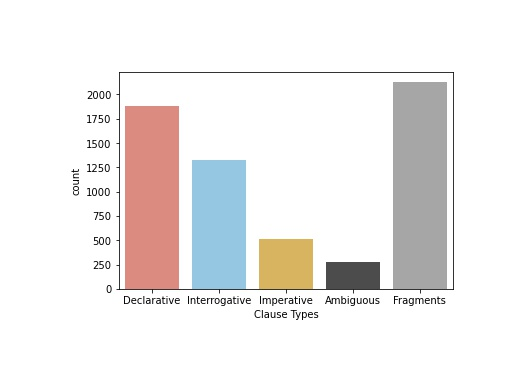
\includegraphics[width=0.7\textwidth]{figures/real-cldist.jpg}
    \caption{Distribution of clause types in the corpus}
    \label{fig:real-cldist}
\end{figure}

Zooming in on interrogatives, \twh-interrogatives are more frequent than polar interrogatives; only 2 cases of disjunctive interrogatives were found in the dataset. Figure~\ref{fig:real-subI} shows the distribution of the subcategories of interrogatives. 

\begin{figure}[H]
    \centering
    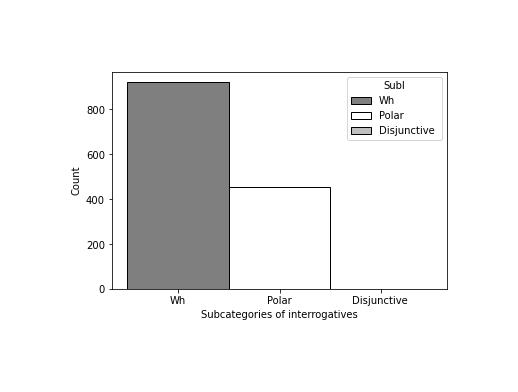
\includegraphics[width=0.7\textwidth]{figures/real-subI.jpg}
    \caption{Subcategories of interrogatives}
    \label{fig:real-subI}
\end{figure}

\begin{figure}[H]
    \centering
    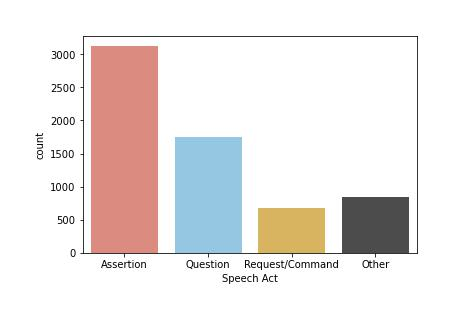
\includegraphics[width=0.7\textwidth]{figures/real-sp.jpg}
    \caption{Distribution of speech acts in the corpus}
    \label{fig:real-sp}
\end{figure}

As shown in Figure~\ref{fig:real-clsp} and \ref{fig:real-spcl}, the three major clause types are mostly used for their canonical functions. The majority of declaratives are used to express assertive force; the majority of interrogatives are used to express question force; and the majority of imperatives are used to express command/request force. 

\begin{figure}[H]
    \centering
    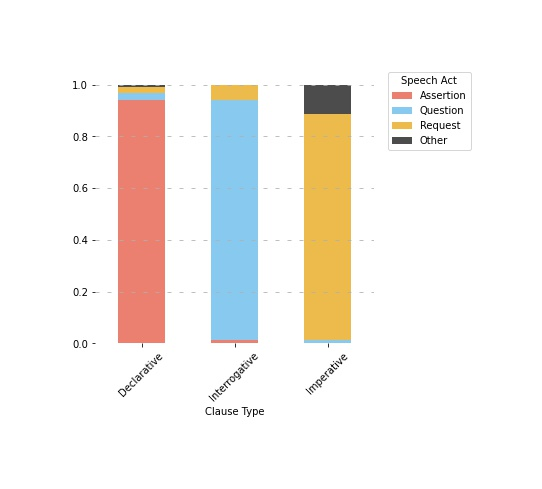
\includegraphics[width=0.7\textwidth]{figures/real-clsp.jpg}
    \caption{The speech acts performed by each clause type in parents' speech}
    \label{fig:real-clsp}
\end{figure}

Conversely, as shown in Figure~\ref{fig:real-spcl}, the majority of assertions are expressed by declaratives, the majority of questions by interrogatives, and the majority of commands/requests by imperatives.

\begin{figure}[H]
    \centering
    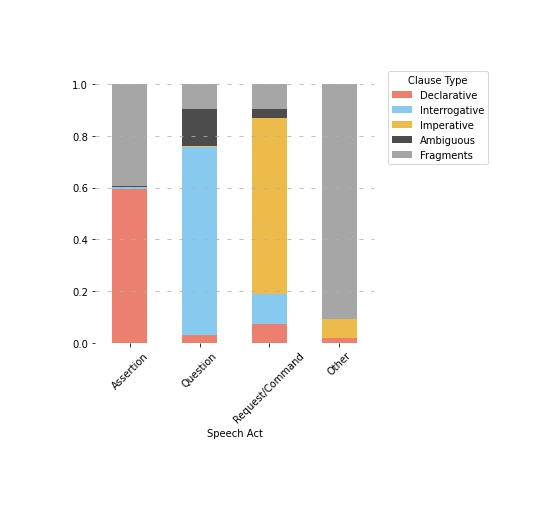
\includegraphics[width=0.7\textwidth]{figures/real-spcl.jpg}
    \caption{The clause type used to express each speech act in parents' speech}
    \label{fig:real-spcl}
\end{figure}


The few cases of mismatches between clause type and force appear to show that such mismatches are systematically marked by morpho-syntactic features, similar to what \textcite{zaitsu2020} have found. For example, declarative and interrogative sentences used for requests/commands tend to have modals, attitude verbs, or future morphology in the sentence:

\bex{eng-cl:dec-req}
\bxl{}	I need you to help me.		\hfill	Mother of William, Session 010605
\ex	Can you say hi?				\hfill	Mother of Lily, Session: 010117
\ex	(previous utterance: I'm gonna do some work.)\\
And you’re gonna do some coloring.\hfill		Mother of Violet, Session: 010407
\ex  Are you gonna read to Mommy?	\hfill	Mother of Lily, Session 010102
\exl
\eex 

Declarative and imperative sentences used as questions are predominantly marked with final rise intonation. We will return to the prosodic features of each clause type in Chapter~\ref{chap:eng-sp}.

%, as in (\ref{eng-cl:dec-rise}a-b), or have embedded interrogatives (\ref{eng-cl:dec-rise}c):
\begin{comment}
\bex{eng-cl:dec-rise}
\bxl{}
Try this again?			\hfill Mother of William, Session 010605
\ex Oh , you don't wanna play with this ? \hfill	Mother of Naima, Session 001126
\ex Tell Mommy what it says. \hfill Mother of Alex, Session 010427 
\exl
\eex

\end{comment}

\begin{figure}[H]
    \centering
    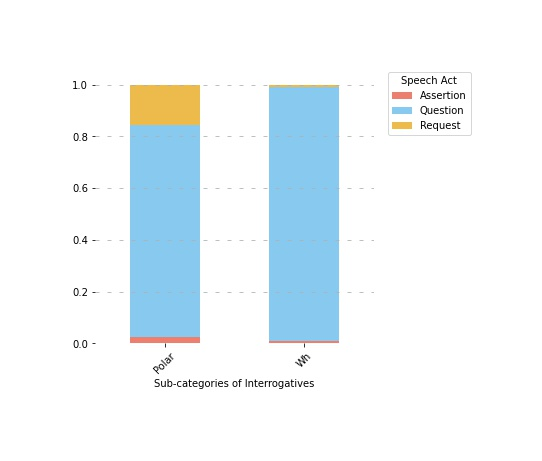
\includegraphics[width=0.7\textwidth]{figures/real-subIsp.jpg}
    \caption{The speech act expressed by different subcategories of interrogatives}
    \label{fig:real-subIsp}
\end{figure}




Turning now to the speech acts expressed by interrogatives, Figure~\ref{fig:real-subIsp} shows the proportion of speech acts that polar and \twh-interrogatives express. The only two examples of disjunctive interrogatives were used both as questions, and are thus not graphed in this figure. Polar interrogatives are used to express more types of speech acts than \twh-interrogatives: around 18\% of polar interrogatives were used for indirect requests like in (\ref{ex:engcl:int-req}) or assertions like in (\ref{ex:engcl:int-asst}):
\bex{ex:engcl:int-req}
Can you give Mommy the ball? \hfill Mother of William, Session: 010412
\eex
\bex{ex:engcl:int-asst}
Doesn’t he have sharp teeth?	\hfill	Mother of Lily, Session: 010611
\eex

Few \twh-interrogatives are used as non-question. We found 4 cases of \twh-interrogatives used to indirectly make a request (\ref{eng-cl:wh-req}), and indirectly making assertions by way of asking rhetorical questions (\ref{eng-cl:wh-asst}):\footnote{We did also find sentences with \tit{how about/what about} (Rawlins and Bledin~2021), but the majority of these sentences do not come with a verb and were considered fragments (\ref{eng-cl:howabout-frag}). But we also found one case of \tit{how about} interrogative with a verb (\ref{eng-cl:howabout-int}), and the primary intention of the utterance is to make a request. 

\begin{xlisti}
\ex \label{eng-cl:howabout-frag} How about this one?	\hfill	Mother of Alex Session 010512
\ex \label{eng-cl:howabout-int} How about we do these babies. \hfill	Mother of Lily, Session 010102
\end{xlisti}
}


\bex{eng-cl:wh-req}
Why don’t you turn around.	\hfill Mother of William, Session 010619
\eex
\bex{eng-cl:wh-asst}
\twh-interrogatives as assertions
\bxl{}
Who doesn’t love cheese?\hfill	Mother of Lily, Session: 010117
\ex Why are there no pens in this family?\hfill	Mother of Violet, Session: 010407
\exl
\eex


In sum, clause types are typically used for their canonical function in the input to children. This suggests that having speech act information could indeed be more helpful than hurtful for learning to categorize clauses into clause types.

\subsubsection{Morpho-syntactic cues}
\label{sec:engcl:corpus:formal}
We now turn to the formal cues of each clause type, as reviewed in Section~\ref{sec:engcl:bg:grammar}. In this analysis, we excluded fragment utterances that only contain a noun (\tit{Birdie!}) or an interjective (\tit{Oh}). In total, 3923 sentences were included in the analysis. The distribution of the morpho-syntactic cues listed in Table~\ref{tab:eng-cl:formal-schema} across different clause types is shown in Figure~\ref{fig:real-syncluster}. Darker colors represent the number of sentences with the morpho-syntactic property, and lighter colors represent sentences without the property.%The x-axis of the figure represents the counts of sentences, and the eight morpho-syntactic features are listed along the y-axis. Each graph is split in the middle: to the left of the line, bars with darker colors represent the counts of declarative, interrogative, or imperative sentences with this specific feature, and to the right, bars with lighter colors represents the number of sentences without this feature. 





\begin{figure}[H]
    \centering
    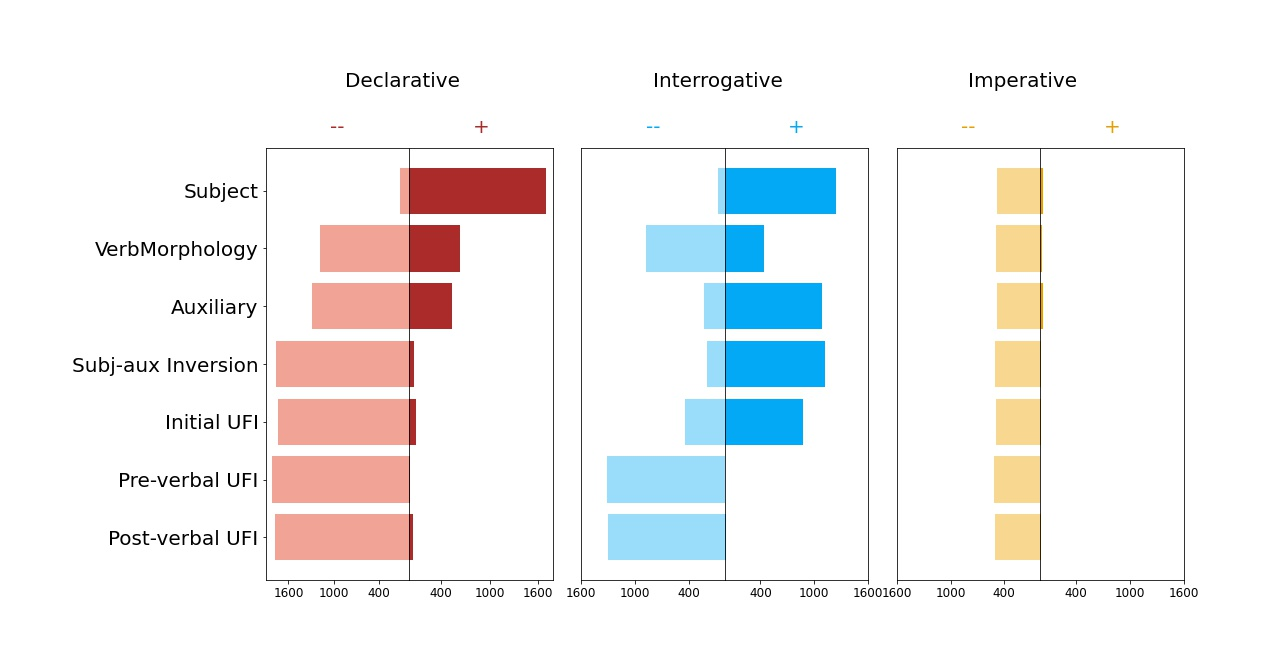
\includegraphics[width=1\textwidth]{figures/real-syncluster.jpg}
    \caption{Number of sentences with/without various formal cues in each clause type; darker colors represent number of sentences with the cue, lighter colors, number of sentences without the cue }
    \label{fig:real-syncluster}
\end{figure}

We can see that the three main clause types have different formal profiles in the input, but the general pattern aligns with the properties of [\textpm int] and [\textpm imp] discussed in Section~\ref{sec:engcl:bg:grammar}: interrogativity is associated with subject-auxiliary inversion and sentence-initial \twh{} (i.e. an unknown functional item for infants); [+imp] is associated with the lack of verb suffixes (i.e. the use of bare verb stems) and subjects; declaratives, the default clause type, are associated with the presence of subjects and verb suffixes, and the lack of subject-auxiliary inversion and clause-initial UFIs. 

From these results, we can see that the formal signatures of each clause type is consistently present in the input: auxiliary-inversion for interrogatives and the lack of subjects and verb suffixes for imperatives. But how informative are these cues to clause typing? And what can or does speech act information add to these cues? In the next section, I train two logistic regression models with actual clause type labels (i.e. using a supervised learning method in machine learning terms) to see how well the models find statistical regularities related to clause typing in the data. 

% However, we do see some features that might not matter for clause typing are also present, such as the presence of subjects in declaratives and interrogatives. 

\subsubsection{Informativeness of syntactic and pragmatic cues}
\label{sec:engcl:corpus:supervised}
In the previous section, we saw that in parents' speech to 18-month-olds, the three clause types are mostly mapped to their canonical functions, and that they have different morpho-syntactic profiles as expected. In this section, I evaluate the informativeness of syntactic and pragmatic cues by comparing two supervised learning models. Unlike the models simulating the \dlearnerabbr{} learner and the \plearnerabbr{} learner I will discuss later, these two supervised models were trained on a subset of our annotated dataset with clause type labels given as input. That is, the models are given correctly annotated data for training (hence the term ``supervised'') and attempt to determine the significant statistical regularities associated with each clause type. After the training phase, these models were tested on the part of data they have not seen, to see how well they could use the statistical regularities discovered in the training data to predict clause type labels. 

The supervised \dlearnerabbr{} model uses morpho-syntactic cues as predictors for clause typing, while the supervised \plearnerabbr{} model uses both morpho-syntactic and speech act information. Both are multinomial logistic regression models trained on 90\% of the annotated dataset, with clause type categories as dependent variable (declarative as the baseline), and a set of morpho-syntactic cues as predictors. As discussed in Section~\ref{sec:engcl:bg:grammar}, [+int] is associated with the presence of cues (e.g. auxiliary inversion, clause-initial \twh{}, complementizer), while [+imp] is associated with the absence of cues (e.g. verb suffix, subject). So the set of syntactic predictors in our models is [-subject, $-$verb suffix, +auxiliary, +subj-aux inversion, +clause-initial UFI,+pre-verbal UFI, +post-verbal UFI]. We then test the performance of both on the unseen 10\% of the data to see how well they predict the clause type categories. We calculated the adjusted rand score of both models to evaluate their performance. The rand index is normally used to measure the similarity between two data clusterings (\cite{rand1971}), calculated by taking all pairs of samples and counting ones that are assigned to the same or different clusters in the predicted and true clusterings:

\begin{equation} \mbox{RI} =\frac{ \mbox{number of agreeing pairs}}{ \mbox{number of pairs}} 
\end{equation}

\revise{The adjusted Rand index (ARI) is the corrected-for-chance version of the Rand index (cf. \cite{hubert1985ari,steinley2004ari}):}

\begin{equation} \label{eq:ari}
\mbox{ARI} =\frac{ \mbox{RI}-\mbox{Expected RI}}{ max(\mbox{RI})-\mbox{Expected RI}} 
\end{equation}


The performance of the two models over 10 iterations is shown in Figure~\ref{fig:super-compare-rand}. Overall, the supervised \praglearner{} outperforms the supervised \distlearner{}, suggesting that the speech act information provides additional information for clause typing.


\begin{figure}[H]
    \centering
    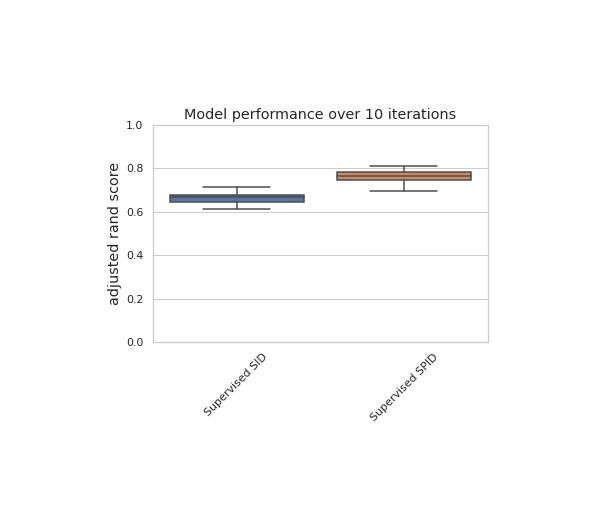
\includegraphics[width=0.8\textwidth]{figures/super-compare-rand-name.jpg}
    \caption{Comparing the two supervised models by rand score (performance over 10 iterations)}
    \label{fig:super-compare-rand}
\end{figure}


%Both models found the same morpho-syntactic regularities the coefficients the two models assigned to the morpho-syntactic predictors 

Our next question is how well the models know the morpho-syntactic makeup of each clause type. This can be inferred from the coefficients that the two models assign to the morpho-syntacitc predictors. A bigger coefficient assigned to a predictor means that the model assigns it a higher significance. As declarative clauses were used as the baseline, the coefficients should in particular be interpreted as indicating how much a specific morpho-syntactic cue contribute to the increase/decrease in the log odds of the sentence being classified as interrogative/imperative vs. declarative (i.e. if a sentence has a morpho-syntactic cue, how likely will it have the feature [+int] or [+imp] as opposed to the default clause type [-int, -imp]). Table~\ref{tab:engcl:corpus:formal} summarizes the morpho-syntactic profile of each clause type. For our purposes, significance was calculated using a two-tail $z$-test. %Details of the models, coefficients, and $p$-values are reported in \mycode{}. 

\begin{table}[H]
\begin{center}
\begin{tabular}{c|p{10cm}}
\hline
Clause Type Feature & Morpho-syntactic cues\\
\hline \hline
Interrogatives (+int) & +auxiliary, +subject-auxiliary inversion, +sentence-initial UFI\\
\hline
Imperatives (+imp) & $-$subject, $-$verb suffix\\
\hline \hline
\end{tabular}
\end{center}
\caption{Morpho-syntactic cues associated with interrogatives and imperatives compared to declaratives}
\label{tab:engcl:corpus:formal}
\end{table}%


As seen in the table, compared to declaratives, interrogatives are more likely to have subject-auxiliary inversions and sentence-initial UFIs; imperatives are more likely to have null subjects and bare verb stems, as expected. Some associations were less expected. For example, [+int] is associated with [+auxiliary], which is not predicted by our theory of clause typing in English. But this in fact reflects another formal property of English [+int], namely \tit{do}-support. Whenever T and V are not syntactically adjacent (either because T to C movement or negation in declaratives and imperatives), \tit{do} is inserted. Since T to C movement is common in interrogatives, but negation is less common in imperatives and declaratives, this elevates the rate of auxiliary in interrogatives relative to the other kinds of clauses. %Since \tit{do} is optional in declaratives and imperatives, but necessary in interrogatives, it is not surprising that auxiliaries appear more often in interrogatives. 

%A more realistic model for infant language learning would be unsupervised model where they discover the clustering of sentences. Nevertheless, the supervised learners are useful as an estimate of how informative formal and speech act features are for the task of inferring clause type.

Of course, these two models do not reflect how infants learn clause typing, as they were given clause type information. Infants must learn clause typing without having access to data of which the clause type label is given. These supervised models are nevertheless useful for appreciating the information contained in the data that children receive as input. They allow us to measure the correlation between the features and clause type categories, which provides an upper limit on how much information could be conveyed by the morpho-syntactic cues.. The results from these two models suggest that the information needed for clause typing is indeed available in the input and, in particular, from the categories with which we annotated our data. In the next section, we will get one step closer to addressing how infants learn clause types by removing the actual clause type labels from our models (switching to what in machine learning is known as ``unsupervised learning''). This makes the learning models more similar to the actual learning task where infants are not given these labels. Using these models, we can ask whether a learner that expects three clause type categories would be able to solve the clustering problem discussed in Chapter~\ref{chap:introduction} on the basis of morpho-syntactic cues alone. We then consider the question of whether adding in speech act information would help. Finally, as speech act information is likely not perceived veridically (e.g. due to developing pragmatic skills at this age), I ask how much pragmatics learners need to learn clause type categories. 


\section{Modeling the learning of clause types}
\label{sec:engcl:model}
Now that we have seen that the relevant information for clause typing is present in the input, our next step is to see whether a learner that can only perceive the morpho-syntactic cues would have enough information to find the right clause types. 

As discussed in Section~\ref{sec:engcl:bg:learners}, I examine the role of pragmatics computationally by building two Bayesian clustering models. The two models simulate a \distlearner{} and a \praglearner{}. Both are distributional learning models: as input, they observe the distribution of several morpho-syntactic cues that are identifiable by infants at 18 months old, and they use that information to cluster sentences into three clause type categories. Given that, cross-linguistically, the same three types of clause types (\diis{}) are associated with three major speech acts (\aqrs{}), it is reasonable to assume that an expectation for three clause types is innate. Even if learners do not have this innate expectation, determining whether learning can succeed with this expectation is a first step in determining whether it is possible to learn the clause types without it. Our learners thus assume that there are three categories, and only have to discover what these categories are, based on formal features. The \praglearner{} additionally observes speech act information and assumes that it is related to clause type. We further manipulated the ratio of noise in the pragmatic information that the pragmatically informed learner is given, to test how much pragmatics the learner needs.


This section is organized as follows. Section~\ref{sec:engcl:model:spec} specifies the generative models simulating the two learners. Then I specify how the two models infer clause type categories in Section~\ref{sec:engcl:model:infer}. Section~\ref{sec:engcl:model:results} reports the simulations with English infant-directed speech demonstrating that pragmatic information is crucial for finding the right clause type clustering, and that this pragmatic information does not have to be perfect, as even with 80\% of noise, it still boosts the performance of the \praglearner{}. 

\subsection{Generative models}
The two models simulating the \distlearner{} and the \praglearner{} are Bayesian clustering models, illustrated in Figure~\ref{fig:engcl:model}.% 

\label{sec:engcl:model:spec}

\begin{figure}[H]
\begin{minipage}[b]{0.45\linewidth}	
\begin{center}
\begin{tikzpicture}
\node[latent] (c) {$c_{i}$};
\node[obs, below=of c, xshift=-0.6cm] (s) {$\vec{s_{i}}$};
\node[latent, left=of c] (phi) {$\phi$};
%\node[const, left=of phi] (beta) {$\beta$};
\node[latent, left=of s] (delta) {$\delta^{(c)}$};
%\node[const, left=of delta] (gamma) {$\gamma$};

\edge {phi}{c};
\edge {delta, c}{s};
%\edge {beta}{phi};
%\edge {gamma}{delta};

\plate {nutt}{(c)(s)}{$N$};
\plate {cvalue}{(delta)}{$C$};
\plate {fvalue}{(delta)(s)(cvalue)}{$F$};
\end{tikzpicture}
\end{center}
%\end{figure}
\end{minipage}
\hspace{0.5cm}
\begin{minipage}[b]{0.45\linewidth}	
%\begin{figure}[H]
\begin{center}
\begin{tikzpicture}
\node[obs] (a) {$a_{i}$};
\node[latent, left=of a] (theta) {$\theta$};
%\node[const, left=of theta] (alpha) {$\alpha$};
\node[latent, below=of a] (c) {$c_{i}$};
\node[obs, below=of c, xshift=-0.6cm] (s) {$\vec{s_{i}}$};
\node[latent, left=of c] (phi) {$\phi^{(a)}$};
%\node[const, left=of phi] (beta) {$\beta$};
\node[latent, left=of s] (delta) {$\delta^{(c)}$};
%\node[const, left=of delta] (gamma) {$\gamma$};

\edge {theta}{a};
%\edge {alpha}{theta};
\edge {phi, a}{c};
\edge {delta, c}{s};
%\edge {beta}{phi};
%\edge {gamma}{delta};

\plate {nutt}{(a)(c)(s)}{$N$};
\plate {avalue}{(phi)}{$A$};
\plate {cvalue}{(delta)}{$C$};
\plate {fvalue}{(delta)(s)(cvalue)}{$F$};
\end{tikzpicture}
\end{center}
\end{minipage}
\caption{The  \distlearner{} (left) and \praglearner{} (right)}\label{fig:engcl:model}
\end{figure}




Both models assume that there are three clause type categories, \diis{}, that explain the distribution of a set of morpho-syntactic properties in the input. This is shown in the graphical illustrations in Figure~\ref{fig:engcl:model} as the morpho-syntactic properties $\vec{s_{i}}$ being conditioned on the clause type variable $\vec{c_{i}}$. The \plearnerabbr{} model additionally assumes that there are four speech act categories (assertions, questions, requests/commands, or some other speech acts such as exclamatives), and that this pragmatic information helps to identify the clause type category. This is shown in the graphical representation as the variable $c_{i}$ being conditioned on the variable $a_{i}$ (for speech act). Tables~\ref{tab:engcl:baseline-variables} and ~\ref{tab:engcl:target-variables} summarize the notation and statistical assumptions for the two models. 

\begin{table}[H]
    \centering
    \begin{tabular}{cl}
    \hline
    \hline
        $c_{i}$ &  Clause type, declarative, interrogative, imperative\\
        &$\vec{\phi^{a}} \sim \mbox{Dir}(1,1,1)$\\        
        & $ c_{i} \sim  \mbox{Multinomial}(\vec{\phi})$;\\
\hline
        $\vec{s_{i}}$ &  Morpho-syntactic properties; \\
        & See Table~\ref{tab:eng-cl:formal-schema} for the full list of features included \\
        &$\delta\sim \mbox{Beta}(1,1)$\\        
        & $s_{i}^{(F)} \sim \mbox{Bernoulli}(\delta^{(c)})$ \\
    \hline
    \hline
    \end{tabular}
    \caption{Variables in \distlearner{} model, their distribution, and explanation}
    \label{tab:engcl:baseline-variables}
\end{table}


\begin{table}[H]
    \centering
    \begin{tabular}{c|l}
    \hline
    \hline
        $a_{i}$ & Speech Act: \\
        	  &Assertion, Question, Request/Command, Other\\
          & $\vec{\theta} \sim \mbox{Dir}(1,1,1,1)$\\
          & $ a_{i} \sim \mbox{Multinomial}(\vec{\theta})$;\\

\hline
         $c_{i}$ &  Clause Type:\\
        & Declarative, Interrogative, Imperative\\
        &$\vec{\phi^{(a)}} \sim \mbox{Dir}(1,1,1)$\\
        &  $c_{i} \sim  \mbox{Multinomial}(\vec{\phi^{(a)}})$;\\
\hline
        $\vec{s_{i}}$ &  Set of morpho-syntactic properties; \\
        $s_{i}^{(F)}$ &  property $F$ in the set;  \\
        &$\delta\sim \mbox{Beta}(1,1)$\\        
        & $s_{i}^{(F)} \sim \mbox{Bernoulli}(\delta^{(c)})$ \\
    \hline
    \hline
    \end{tabular}
    \caption{Variables of the \plearnerabbr{} model, their distributions, and explanations}
    \label{tab:engcl:target-variables}
\end{table}






In both models, the clause type variable $c_{i}$ follows a multinomial distribution with a parameter $\phi$. This parameter is assumed to have a uniform Dirichlet prior $\mbox{Dir}(1,1,1)$. This means that it is equally likely \emph{a priori} for a sentence to be a declarative, interrogative or imperative. For the model simulating the \distlearner{}, the parameter $\phi$ represents the probability that a sentence $i$ is a declarative, interrogative, or imperative. As the \plearnerabbr{} model assumes that the speech act category $a_{i}$ of the utterance expressed by the sentence informs the learner of the clause type category, so the parameter $\phi^{(a)}$ in this model represents the probability that a sentence $i$, which expresses the speech act $a_{i}$, is a declarative, interrogative, or imperative. 

In the \plearnerabbr{} model, the speech act variable $a_{i}$ follows a multinomial distribution with parameter $\theta$. This parameter represents the probability that the speech act expressed by the sentence $i$ is an assertion, question, request/command, or some other speech act. This parameter also has a uniform Dirichlet prior $\mbox{Dir}(1,1,1,1)$, meaning that we assume that it is equally likely \emph{a priori} that the sentence $i$ expresses an assertion, question, request/command, or some other speech act.

In both models, morpho-syntactic properties are represented by a vector of Bernoulli variables $\vec{s_{i}}$, and $\vec{s_{i}}$ is conditioned on $c_{i}$. 
The number of morpho-syntactic properties included is represented by a vector $F$, and the properties are the same as the ones in the corpus study listed in Table~\ref{tab:eng-cl:formal-schema} in Section~\ref{sec:engcl:corpus:schema}. Each $s^{(F)}_{i}$ in $\vec{s_{i}}$ takes the value 1 if the sentence contains the property, and 0 otherwise. $s^{(F)}_{i}$ is conditioned on the parameter $\delta^{(c, F)}$, which represents the probability of observing a given morpho-syntactic property in a particular clause type category. 
This parameter is assumed to have a uninformative uniform $\mbox{Beta}(1,1)$ prior, meaning that \tit{a priori}, it is equally likely for a particular property to be present or absent in a clause type category. 



\subsection{Inferences}
\label{sec:engcl:model:infer}

The task of both learners is then to infer the category assignment of the clause type variable (i.e. is the sentence a declarative, interrogative, or imperative) from observations of morpho-syntactic properties of the sentence. The \plearnerabbr{} learner additionally observes speech act information and assumes it is related to clause type. 

I applied Gibbs sampling (\cite{geman1984gibbs}), a form of a Markov chain Monte Carlo sampler to sample from the posterior distribution of clause type category assignments. The sampling algorithm of the two learners are detailed below. In the following algorithms, $\vec{c}$ represent the set of clause type assignments in the corpus. The variable $\vec{a}$ represents the set of all speech act values in the corpus; $\vec{S}$ represents all values in the corpus for the set of morpho-syntactic properties, and $\vec{s^{(F)}}$ represents all the values in the corpus for a specific morpho-syntactic feature $F$. The subscript $i$ represents the current sentence, and $-i$ represents all values of a variable except the current sentence (for example, $c_{i}$ represents the clause type assignment of the current sentence, and $c_{-i}$ represents the clause type assignments of all sentences in the corpus except the current one). The following counts are calculated:
\bex{}
$n$ is total number of observations so far;

$n_{c_{i}}$ is the number of observations of $c = c_{i}$ so far;

$n_{a_{i}}$ is the number of observations of $a = a_{i}$ so far;

$n^{(a_{i})}_{c_{i}}$ is the number of observations of $c=c_{i}$ while $a = a_{i}$;

$n^{(F,c_{i})}_{s_{i}}$ is the number of observations so far where $s^{(F)}=1$ when $c = c_{i}$;

$n^{(F)}_{c_{i}}$ is the number of observations of feature $F$ so far when $c = c_{i}$
\eex

\begin{comment}
\tbf{The \dlearnerabbr{} model:} We first randomly initialized assignments of $c_{i}$ for each sentence with three categories (representing declaratives, interrogatives, and imperatives). 

\tbf{The \plearnerabbr{} model:} The algorithm first randomly initializes assignments of $c$ for all sentence with three values (representing declaratives, interrogatives, and imperatives). Then it sweeps to update values of $c_{i}$. The likelihood term of both models is the conditional probability $p(\vec{S}|\vec{c})$. The prior terms differ, as for the \plearnerabbr{} the probability of the assignment of $c_{i}$ is conditioned on the speech act values $\vec{a}$. The posterior predictive probability can be computed using Bayes' Rule as follows:

\begin{equation}
p(c_{i}| c_{-i}, \vec{a}, \vec{S_{i}},\phi, \delta) = \frac{p(\vec{S_{i}}| \vec{c}, \delta)\ p(c_{i}|, c_{-i}, \phi,\vec{a})}{\Sigma_{c_{i}'}p(\vec{S_{i}}| \vec{c'}, \delta)\ \ p(c_{i}'|, c_{-i}, \phi, \vec{a})}
\end{equation}

%The prior distribution $ p(c_{i}|, c_{-i}, \vec{a})$ follows a Multinomial distribution with the parameter $\phi$, which in turn follows a Dirichlet distribution with parameter $\beta$:

\begin{equation}
\begin{split}
 p(c_{i}|\phi_{a_{i}} ,\beta, c_{-i},  \vec{a})  =& \int p(c_{i}|\phi_{a_{i}}, \beta) p(\phi_{a_{i}}| c_{-i}, \beta)d\phi_{a_{i}} \\
= & \int \prod_{k}\ \phi_{k}^{1^{c_{i}=k}}\ \frac{\Gamma(\sum_{k}\beta_{k})}{\prod_{k}(\Gamma(\beta_{k}))}\prod_{k} \phi_{k}^{\beta_{k}-1}d\phi
\end{split}
\end{equation}

The likelihood term:

\begin{equation}
\begin{split}\label{p(s|c)}
p(\vec{S_{i}}| \vec{c}, \delta, \gamma) = & \prod_{F} p(s^{(F)}_{i}|\vec{c}^{(F)}, \delta, \gamma)\\%split to each feature of S
= &\prod_{F}\int p(s^{(F)}_{i}|c_{i}^{(F)}, \delta^{(F)}_{c_{i}}, \gamma^{(F)})\ p(\delta^{(F)}_{c_{i}}|c^{(F)}_{-i}, s^{(F)}_{-i},\gamma^{(F)}) d\delta_{c_{i}}\\%predicative posterior distribution
=& \prod_{F}\int \prod_{k} \delta^{1^{s_{i}=k}}_{k}%expand p(s_{i})
\prod_{k} \delta_{k}^{\gamma_{k}-1}  %expand p(delta)
\frac{\Gamma(\sum_{k}(\gamma_{k}))}{\prod_{k}(\Gamma(\gamma_{k}))}%normalizing constant for p(delta)
d\delta_{c_{i}} 
\end{split}
\end{equation} 
\begin{equation}
\begin{split}
p(\vec{S_{i}}| \vec{c}, \delta, \gamma)=&\prod_{F}\frac{\Gamma(\sum_{k}(\gamma_{k}))}{\Gamma(\gamma_{s_{i}})\prod_{k\neq s_{i}}(\Gamma(\gamma_{k}))}%old NC
\frac{\Gamma(\gamma_{s_{i}}+1)\prod_{k\neq s_{i}}(\Gamma(\gamma_{k}))}{\Gamma(\sum_{k}(\gamma_{k})+1)}\\%separate out k from s_{i}
=&\prod_{F}\frac{\gamma_{s_{i}}}{\sum_{k}(\gamma_{k})}\\%reduce
=&\prod_{F}\frac{\gamma_{0}+n_{s_{i}}}{(\gamma_{0}+n_{s_{i}})(\gamma_{0}+n_{c_{i}}-n_{s_{i}})}\\%update function
=& \prod_{F}\frac{\gamma_{0}+n_{s^{F, c_{i}}_{i}}}{2\gamma_{0}+n^{F}_{c_{i}}}
\end{split}
\end{equation}
\end{comment}
   %Assume $\beta_{k}$ is the value of $\beta$ for when $c = k$ (i.e. the clause type assignment is $k$), $n_{c_{i}}$ as the number of observations of $c=c_{i}$ so far, and  $n_{c_{i}}^{(k)}$ is the number of observations of other values of $c$ 

For both models, we first randomly initialize values of $c_{i}$ for each sentence with three categories (representing declaratives, interrogatives, and imperatives). After initialization, the \dlearnerabbr{} sweeps to update current $c_{i}$ with the posterior distribution specified in Equation~\ref{eq:engcl:base}, and the \plearnerabbr{} updates with Equation~\ref{eq:engcl:target}.  

\begin{equation} \label{eq:engcl:base}
\begin{split}
p(c_{i}| c_{-i}, \vec{S_{i}}) = &\frac{p(\vec{S_{i}}| \vec{c})\ p(c_{i}|\beta, c_{-i})}{\Sigma_{c_{i}'}p(\vec{S_{i}}| \vec{c'})\ \ p(c_{i}'| c_{-i})}\\
= & \frac{ \prod_{F}\frac{1+n_{s^{(F, c_{i})}_{i}}}{2+n_{c^{F}_{i}}}%S
\frac{1+n_{c_{i}}}{4+n}%C
}%分子
{\sum_{c'_{i}}\prod_{F}\frac{1+n^{(F, c'_{i})}_{s_{i}}}{2+n^{(F)}_{c'_{i}}}%S
\frac{1+n_{c'_{i}}}{4+n} %C
}%分母
\end{split}
\end{equation}

\begin{equation} \label{eq:engcl:target}
\begin{split}
p(c_{i}| c_{-i}, \vec{a}, \vec{S_{i}}, \delta) = &\frac{p(\vec{S_{i}}| \vec{c})\ p(c_{i}|\beta, c_{-i}, \vec{a})}{\Sigma_{c_{i}'}p(\vec{S_{i}}| \vec{c'})\ \ p(c_{i}'| c_{-i}, \vec{a})}\\
= & \frac{ \prod_{F}\frac{1+n_{s^{(F, c_{i})}_{i}}}{2+n_{c^{(F)}_{i}}}%S
\frac{1+n_{c_{i}}^{(a_{i})}}{4+n_{a_{i}}}%C
}%分子
{\sum_{c'_{i}}\prod_{F}\frac{1+n^{(F, c'_{i})}_{s_{i}}}{2+n^{(F)}_{c'_{i}}}%S
\frac{1+n_{c'_{i}}^{(a_{i})}}{4+n_{a_{i}}} %C
}%分母
\end{split}
\end{equation}



%uses the the observed values of morpho-syntactic properties to infer for the current utterance and the values of $C$ of other sentences to calculate a posterior distribution over new category assignments for the current sentence, and then re-sample the new value of $C$ from this posterior probability distribution. 


For each model, I ran the chain for 5000 iterations and analyzed the last sample. Each learner was simulated 10 times. 


\subsection{Simulations with infant-directed speech}
\label{sec:engcl:model:results}

The data for this model were taken from the annotated dataset reported in Section~\ref{sec:engcl:corpus}. The labels of speech acts and morpho-syntactic observations were used as input to the models, and the true labels of clause type were used to evaluate the performance of the models. As the learners need to use the surface features of sentences to learn about clause-level properties, instead of one-noun utterances or utterances of only injectives, we eliminated from the dataset sentences that do not contain a verb or an auxiliary. In total, $3923$  sentences were fed into the models.


Figure~\ref{fig:compare-rand} shows the adjusted rand scores of the two models over 10 iterations, and in comparison with the adjusted rand scores of the two multinomial logistic regression models ran in Section~\ref{sec:engcl:corpus:supervised}. 
As explained in the last section, this score ranges between 0 and 1, with higher scores indicating better performance. 

Overall, the \plearnerabbr{} model substantially outperforms the \dlearnerabbr{} model. The pragmatic information led to an improvement from an average \revise{0.4 adjusted rand score to an average of 0.7 rand score}, bringing the model up to the level of supervised performance. This suggests that pragmatic information is crucial for learning the clustering of clause type information. 


\begin{figure}[H]
    \centering
    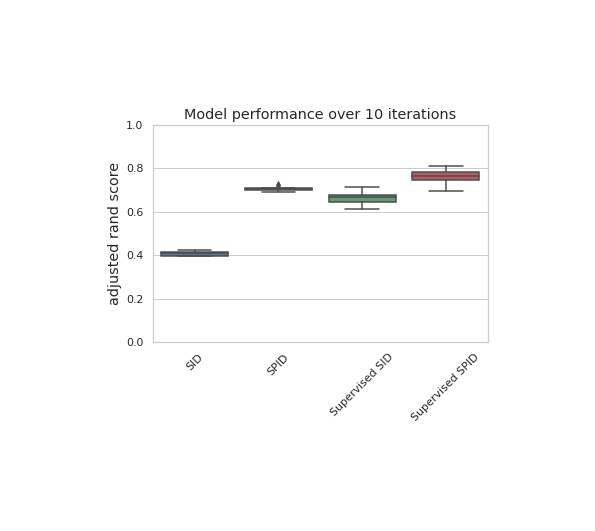
\includegraphics[width=0.8\textwidth]{figures/compare-all-rand.jpg}
    \caption{Comparing all four learners (distributional, pragmatic distributional, supervised distributional, supervised pragmatic) by \revise{adjusted rand score} }
    \label{fig:compare-rand}
\end{figure}


\subsubsection{The \dlearnerabbr{} model}
\label{sec:engcl:model:results:d}
For a model to be successful it is not sufficient that it categorizes its input sentences into \emph{any} three categories. The three categories should correspond to the sets of actual declaratives, actual interrogatives and actual imperatives. That is, for example, if in the classification learned by the model, the actual declaratives are split across two categories, the model has not learned to cluster by clause type.
Turning to the profile of each cluster identified by the \dlearnerabbr{} model, Figure~\ref{fig:baseline-heatmap} shows the proportion of \diis{} in each identified cluster, and Figure~\ref{fig:baseline-heatrev} shows the proportion of sentences clustered together. In other words, Figure~\ref{fig:baseline-heatmap} shows whether each cluster mostly consists of one clause type, and Figure~\ref{fig:baseline-heatrev} shows whether each clause type is put in one cluster.  



\begin{figure}[H]
    \centering
    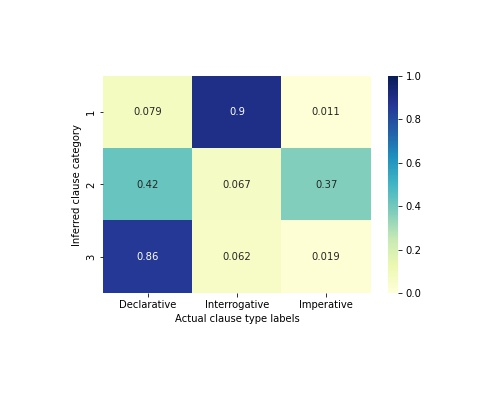
\includegraphics[width=0.7\textwidth]{figures/baseline-heatmap.jpg}
    \caption{The proportion of \diis{} in each of the three clusters identified by the \dlearnerabbr{} model}
    \label{fig:baseline-heatmap}
\end{figure}


\begin{figure}[H]
    \centering
    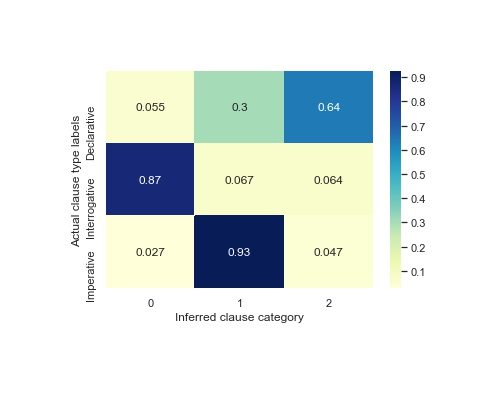
\includegraphics[width=0.7\textwidth]{figures/baseline-heatrev.jpg}
    \caption{The proportion of actual \diis{} clustered in one category}
    \label{fig:baseline-heatrev}
\end{figure}


Overall, Figure~\ref{fig:baseline-heatmap} shows that the \dlearnerabbr{} model identifies an interrogative cluster and a declarative cluster. \revise{Cluster~$1$} mostly contains interrogative clauses, as 90\% of sentences in this cluster are interrogative; \revise{Cluster~$3$} is mostly declarative, and 86\% of the data in this cluster are declaratives. \revise{Cluster~$2$ }is split between declaratives and imperatives. Figure~\ref{fig:baseline-heatrev} shows that 87\% of interrogatives and 93\% of imperatives are clustered together in \revise{Cluster~$1$ and $2$ }respectively. While most of declaratives are classified in \revise{Cluster~$3$}, a proportion is classified in \revise{Cluster~$2$}.

These results seem to suggest that the \dlearnerabbr{} model found one out of three clause types, but how do these clause types look like? Did the model find the right morpho-syntactic properties to associate with each clause type? Figure~\ref{fig:baseline-syncluster} plots the morpho-syntactic profile of each cluster identified by the \dlearnerabbr{}. Darker colors represent sentences with the morpho-syntactic property, and lighter colors represent sentences without the property. 

\begin{figure}[H]
    \centering
    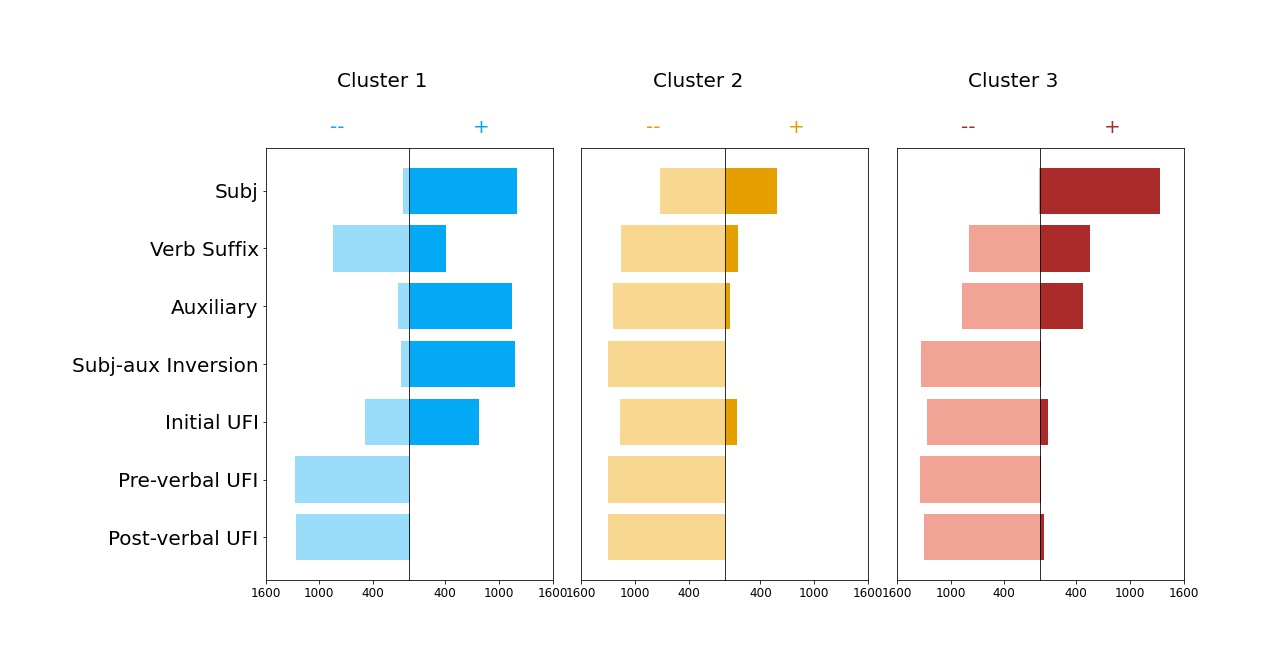
\includegraphics[width=1\textwidth]{figures/baseline-syncluster.jpg}
    \caption{The number of sentences with/without certain formal features in each cluster (\revise{Cluster 1 $\sim$ Interrogatives, Cluster 2 $\sim$ Imperatives, Cluster 3 $\sim$ Declaratives}), darker colors represent the number of sentences with the feature. UFI stands for Unknown Functional Item (e.g. \twh{}), see Table~\ref{tab:eng-cl:formal-schema} for details.}
    \label{fig:baseline-syncluster}
\end{figure}

We can see that \revise{Cluster~$1$}, which is 90\% interrogative clauses, is associated with [+int] morpho-syntactic properties such as subject-auxiliary inversion and sentence-initial unknown functional item (e.g. \twh-phrases). 

The other two clusters are not as ideal. \revise{Cluster~$2$} consists of a mix of imperative sentences and simple declarative sentences. While it appears that the cluster mostly consists of sentences with bare verb stem, which is characteristic for imperatives in English, but a quick look at the sentences show that it also includes declaratives with these properties as well:

\bex{engcl:baseline:cluster1-dec}
 I love school. \hfill Mother of Lily, Session 010423
\eex

The sentence is clustered together with imperatives like \tit{Take the bottle!} by the model. Ambiguous sentences like \ref{engcl:baseline:cluster1-amb} are also put in this cluster:
\bex{engcl:baseline:cluster1-amb}
Wanna read your little Tigger book? \hfill Mother of Violet, Session 010407
\eex

Moreover, compare to the distribution of morpho-syntactic features of imperatives in English in Figure~\ref{fig:real-syncluster}, this cluster seems to have more sentences with subjects. It seems that instead of finding a cluster for imperatives and declaratives, the model puts too much weight on the lack of subjects in a sentence, so any sentences without subjects are in \revise{Cluster~$2$}. 

\begin{comment}
A multinomial logistic regression model was performed to further probe into the morpho-syntactic profile of each cluster, with the three
clusters as dependent variable (with Cluster~$2$ as the default), and the set of morpho-syntactic properties as independent variable. The results are shown in Table~\ref{tab:baseline-synstats} (details of the regression model, coefficients, and $p$-values are reported in Appendix~\ref{appx:engcl}).


\begin{table}[H]
\begin{center}
\begin{tabular}{c|p{10cm}}
\hline
Clusters (default Cluster~$2$) & Morpho-syntactic cues\\
\hline \hline
Cluster~$0$ & +auxiliary, +subject-auxiliary inversion, +sentence-initial UFI\\
\hline
Cluster~$1$  & $-$subject, $-$verb suffix\\
\hline \hline
\end{tabular}
\end{center}
\label{tab:baseline-synstats}
\end{table}%

The table shows that while 
\end{comment}

Overall, the \dlearnerabbr{} model fails to identify the clause type clustering in English, and fails to identify the characteristic morpho-syntactic properties for these clause types. 


\subsubsection{The \plearnerabbr{} model}
\label{sec:engcl:model:results:p}

Figure~\ref{fig:target-heatmap} shows the proportion of \diis{} in each identified cluster, and Figure~\ref{fig:target-heatrev} shows the proportion of sentences clustered together. 
\begin{figure}[H]
    \centering
    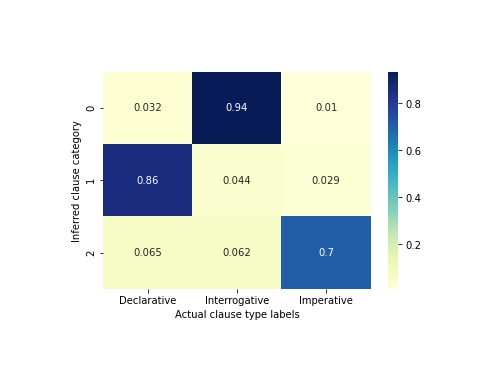
\includegraphics[width=0.7\textwidth]{figures/target-heatmap.jpg}
    \caption{The proportion of \diis{} in each of the three clusters identified by the \plearnerabbr{} model}
    \label{fig:target-heatmap}
\end{figure}




\begin{figure}[H]
    \centering
    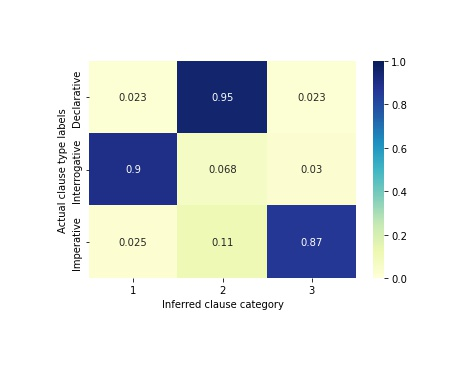
\includegraphics[width=0.7\textwidth]{figures/target-heatrev.jpg}
    \caption{The proportion of actual \diis{} clustered in one category}
    \label{fig:target-heatrev}
\end{figure}
%Rand comparison

%confusion matrix

We can see that the \plearnerabbr{} model clearly identifies a declarative, an interrogative, and an imperative cluster: \revise{94\% of Cluster~$1$ are interrogatives, 86\% of Cluster~$2$ are declaratives, and 70\% of Cluster~$3$ are imperatives.} The three clause types in English are also mostly clustered together by the model: 95\% of declaratives, 90\% of interrogatives, and 87\% of imperatives are clustered together in \revise{Cluster~$2$, $1$, $3$} respectively. In contrast to \dlearnerabbr{} model, this model is able to find the right clause types in English.


Figure~\ref{fig:target-syncluster} shows the morpho-syntactic profile of each cluster identified by the \plearnerabbr{}. 

\begin{figure}[H]
    \centering
    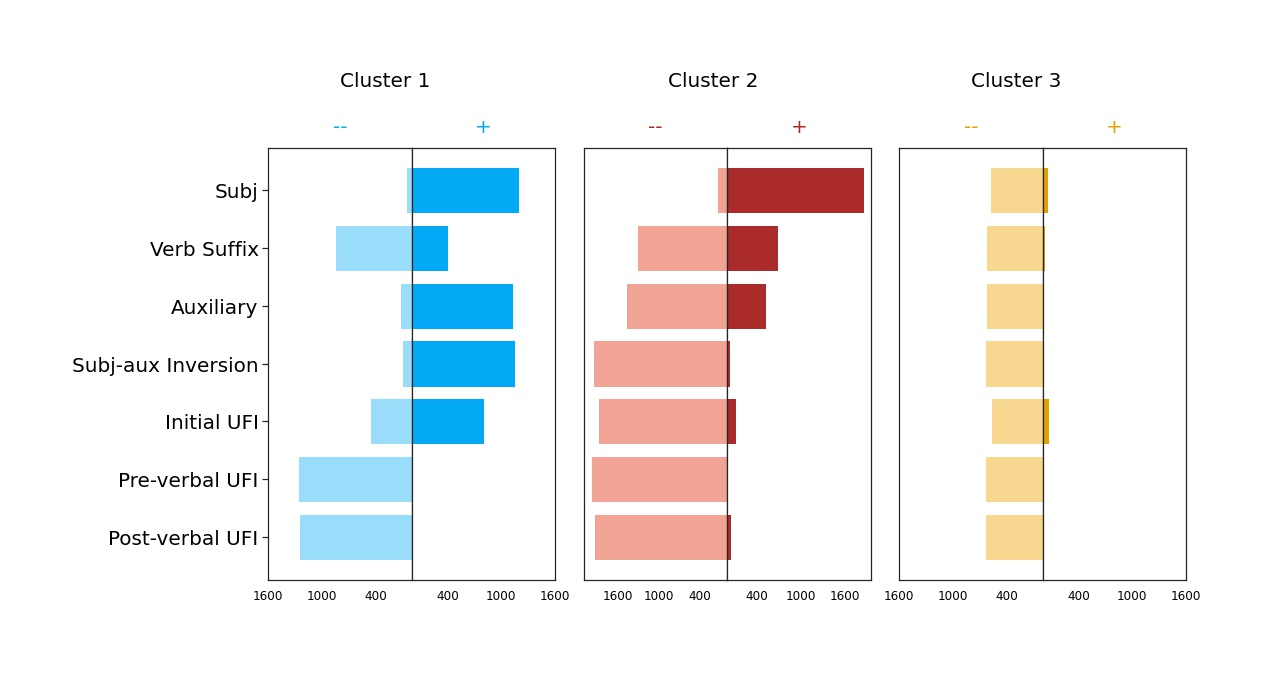
\includegraphics[width=1\textwidth]{figures/target-syncluster.jpg}
    \caption{The number of sentences with/without a formal propertyin each cluster (\revise{Cluster 1 $\sim$ Interrogatives, Cluster 2 $\sim$ Declaratives, Cluster 3 $\sim$ Imperatives}), darker colors represent the number of sentences with the property, lighter colors represent sentences without the property.}
    \label{fig:target-syncluster}
\end{figure}

The profile of the three clusters resembles the profile of \diis{} in our corpus study (Figure~\ref{fig:real-syncluster}). The cluster for interrogatives has more sentences with subject-auxiliary inversion and clause-initial unknown functional items (e.g. \twh{}), and the cluster for imperatives is characterized by the lack of subjects and verb suffixes. 

\begin{comment}
Table~\ref{tab:target-synstats} summarises the three logistic regression models with each of the clusters as dependent variable, and the set of formal features (+/- verb and pre-verbal UFI are excluded, due to low variance) as independent variables.  
\begin{table}[H]
\begin{center}
\begin{tabular}{r|l|l|l}
\hline
 & Cluster~$0$   & Cluster~$1$   &  Cluster~$2$ \\
 & $\sim$ Interrogatives  & $\sim$Declaratives  & $\sim$ Imperatives \\
 \hline\hline
constant & -6.3*** & -1.44*** & 1.95*** \\
\hline
Subject & 0.9** & 4.32*** & -4.75*** \\
\hline
Verb Morphology & -0.31 & 1.66***  & -3.08*** \\
\hline
Auxiliary & 2.66***  & -0.85*** & -2.14*** \\
\hline
Subject-Aux Inversion &5.99*** & -5.83*** & -56.79 \\
\hline
Sentence-initial UFI & 3.65*** & 0.38* & 0.72** \\
\hline
Post-verbal UFI & -0.43  & 0.5  & -1.12 \\
\hline \hline
\end{tabular}
\end{center}
\caption{Results from the three logistic regression models with each of the clusters as the dependent variable and the morpho-syntactic features as independent variables; asterisks represent the significance level: ‘***’ 0.001 ‘**’ 0.01 ‘*’ 0.05 ‘.’ 0.1 ‘ ’ 1}
\label{tab:target-synstats}
\end{table}%
\end{comment}
% \begin{figure}[H]
%     \centering
%     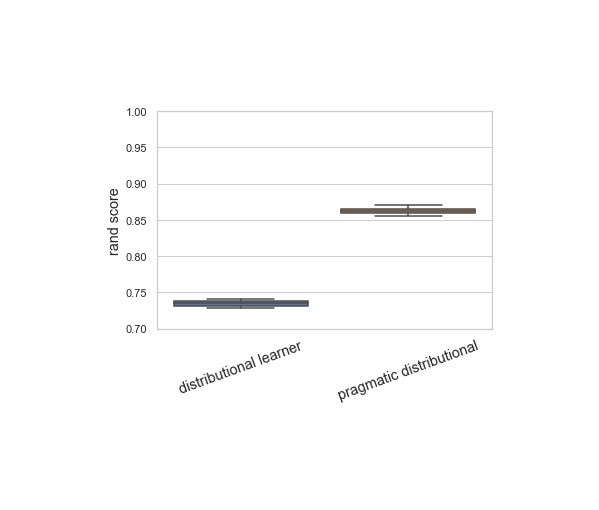
\includegraphics[width=0.6\textwidth]{figures/target-base-rand.jpg}
%     \caption{Comparing the pragmatic distributional learner and the distributional learner by rand score }
%     \label{fig:target-base-rand}
% \end{figure}

\subsubsection{Interim Summary}
\label{sec:engcl:model:results:summary}

Using data from infant-directed speech in English, our models simulate the \distlearner{} and the \praglearner{}.
 We found that the \plearnerabbr{} model performs much better than the \dlearnerabbr{} model; it successfully identifies three clause clusters roughly corresponding to the three major clause types in English. In contrast, the \dlearnerabbr{} model fails to find the right clustering, collapsing declaratives and imperatives. These results suggest that pragmatic information is essential for children to solve the clustering problem for clause types. But how much pragmatics does the learner need? Recall from Chapter \ref{chap:introduction} that assuming \emph{too much} pragmatics to be available to learners might catch us in a circularity. Considering the fact that 18-month-olds' pragmatic skills might still be developing, it is likely that they are not able to perfectly identify the speech act information of some utterances, and thus the pragmatic information available to the learner might be rather noisy. To probe deeper into this question, I now turn to simulated pragmatic learners with noisy speech act information. Studying such learners will allow us to investigate how much pragmatics is need to solve the clustering problem. 



\subsection{Simulating noisy pragmatic information} 
\label{sec:engcl:model:noisy}
%how noise is generated
As we have seen in the last section, pragmatics information is crucial for clause type clustering. In this series of simulations, I manipulated the amount of noise in the speech act information that the \plearnerabbr{} model takes as input. Instead of feeding the model true speech act labels, I replaced a percentage of the data with random speech act labels to simulate the situation where the learner randomly guess the speech act for a proportion of the utterances they hear. Each simulation was run 10 times. 

Figure~\ref{fig:noisy-rand-compare} shows the simulations with 0-100\% noise. The performance of the \dlearnerabbr{} model in our last simulation is indicated by the dotted line. As can be seen, the \plearnerabbr{} learner outperforms the \dlearnerabbr{} learner up until there is around 80\% of noise in speech act, and even at 80\% level there are iterations that outperforms the \dlearnerabbr{}. This suggests that a little pragmatics goes a long way, as the learners with noisy pragmatic information still outperforms the one without. 

\begin{figure}[H]
    \centering
    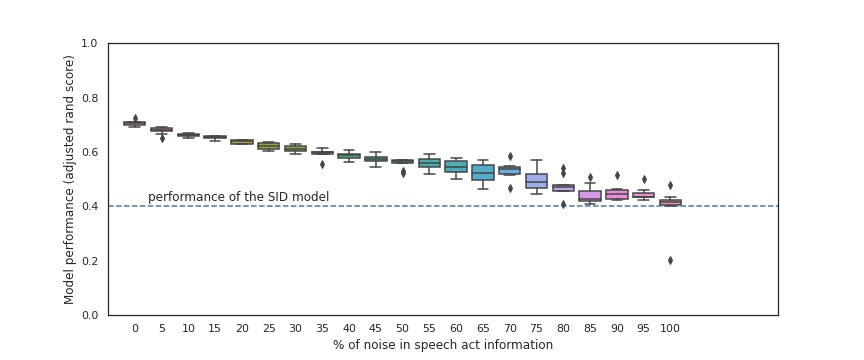
\includegraphics[width=1\textwidth]{figures/noisy-adjrand.jpg}
    \caption{Performance of the \plearnerabbr{} model with different levels of noise in the speech act information; dotted line indicates the \revise{adjusted rand score} of the \dlearnerabbr{} learner}
    \label{fig:noisy-rand-compare}
\end{figure}

\revise{Zooming in on the clusters identified by the models, I found that simulations with around 80\% noise cannot successfully identify all three clusters correctly while simulations with 70\% noise level can, even though the adjusted rand scores of these two levels are roughly the same. At 80\%, we can see that the \plearnerabbr{} reverts back to the performance of the \dlearnerabbr{} in that it fails to identify a cluster for declaratives (Figure~\ref{fig:noisy80-heatmap}). Similar to the \dlearnerabbr{} model, the cluster containing most imperatives also contains many declaratives (\ref{fig:noisy80-heatrev}). }

\begin{figure}[H]
\begin{minipage}[b]{0.45\linewidth}	
    \centering
    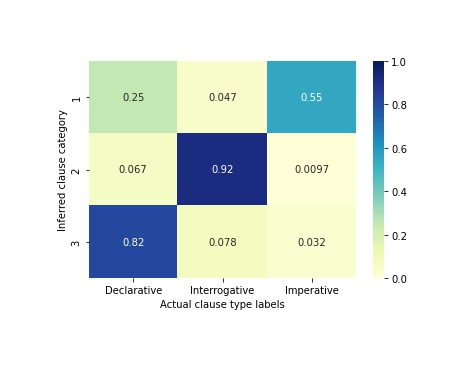
\includegraphics[width=1.2\textwidth]{figures/target-heatmap-70.jpg}
\end{minipage}
\begin{minipage}[b]{0.45\linewidth}	
\centering
    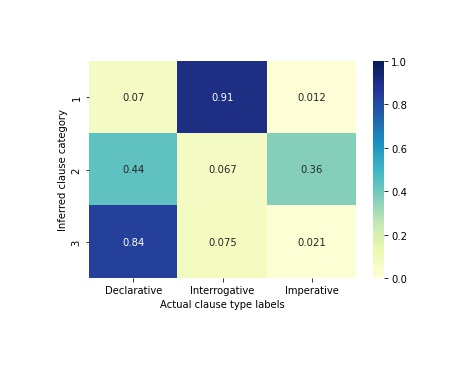
\includegraphics[width=1.2\textwidth]{figures/target-heatmap-80.jpg}
\end{minipage}
    \caption{The proportion of \diis{} in each of the three clusters identified by the \plearnerabbr{} model; with 70\% (left) and 80\% (right) noise in speech act information }
    \label{fig:noisy80-heatmap}
\end{figure}

\begin{figure}[H]
\begin{minipage}[b]{0.45\linewidth}	
    \centering
    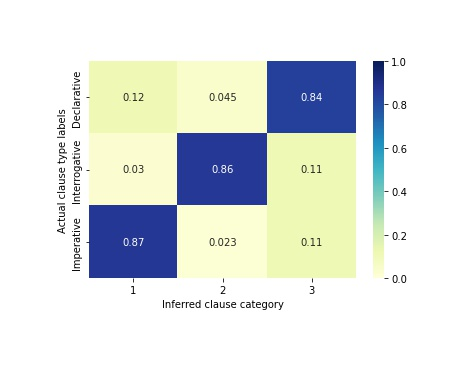
\includegraphics[width=1.2\textwidth]{figures/target-heatrev-70.jpg}
\end{minipage}
\begin{minipage}[b]{0.45\linewidth}	
    \centering
    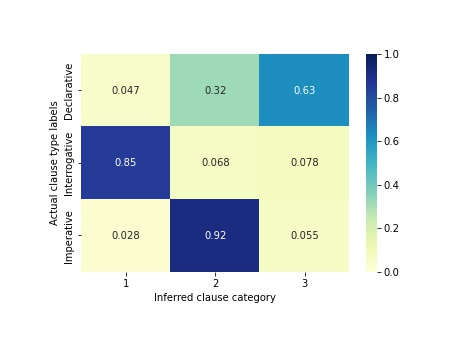
\includegraphics[width=1.2\textwidth]{figures/target-heatrev-80.jpg}
\end{minipage}   
    \caption{The proportion of actual \diis{} clustered in one category, with 70\% (left) 80\% (right) noise in speech act information}
    \label{fig:noisy80-heatrev}
\end{figure}



\revise{The morpho-syntactic profile of different simulations further shows that at 80\% noise level, the \plearnerabbr{} and \dlearnerabbr{} model behave similarly, as both fail to identify the property [$-$ subject] for imperatives (Figure~\ref{fig:noisy80-syncluster}). In contrast, with 70\% noise level the model can still find the right morpho-syntactic features for interrogatives and imperatives (Figure~\ref{fig:noisy70-syncluster}).} 

\begin{figure}[H]
    \centering
    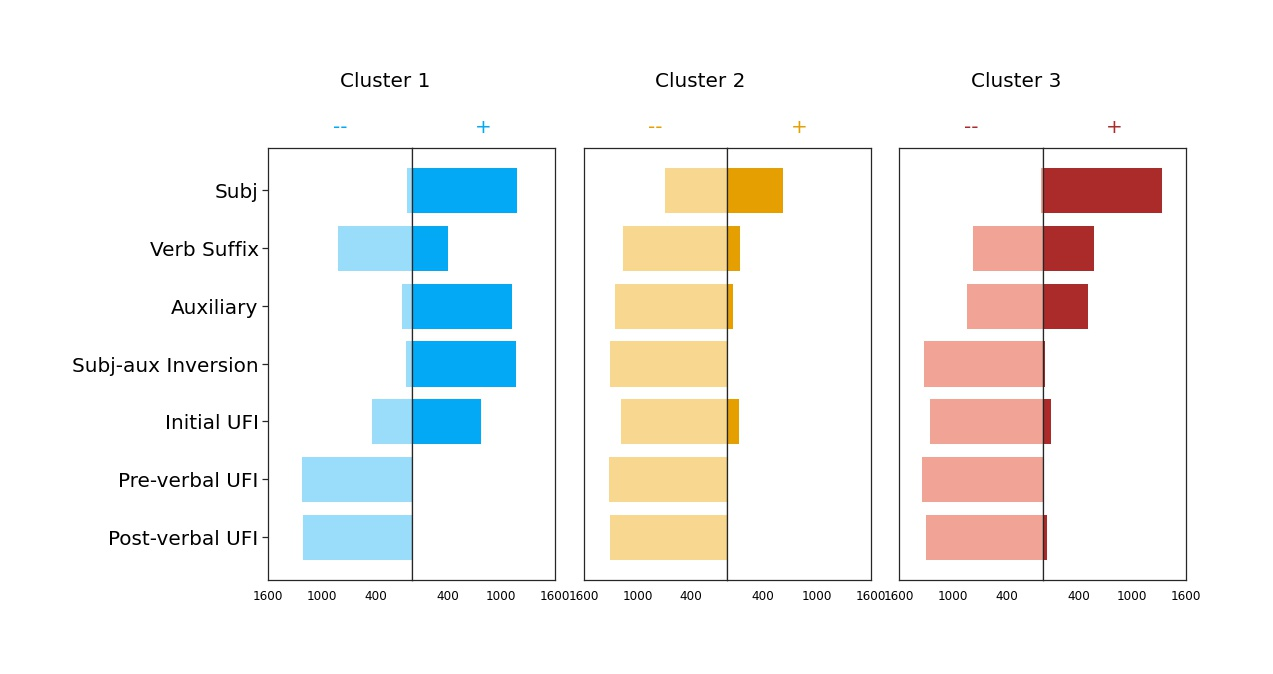
\includegraphics[width=1\textwidth]{figures/target-syncluster-80.jpg}
    \caption{\revise{The morpho-syntactic profile of each cluster in simulations with 80\% noise in speech act information (Cluster 1 $\sim$ Imperatives, Cluster 2 $\sim$ Interrogatives, Cluster 3 $\sim$ Declaratives).}}
    \label{fig:noisy80-syncluster}
\end{figure}

\begin{figure}[H]
    \centering
    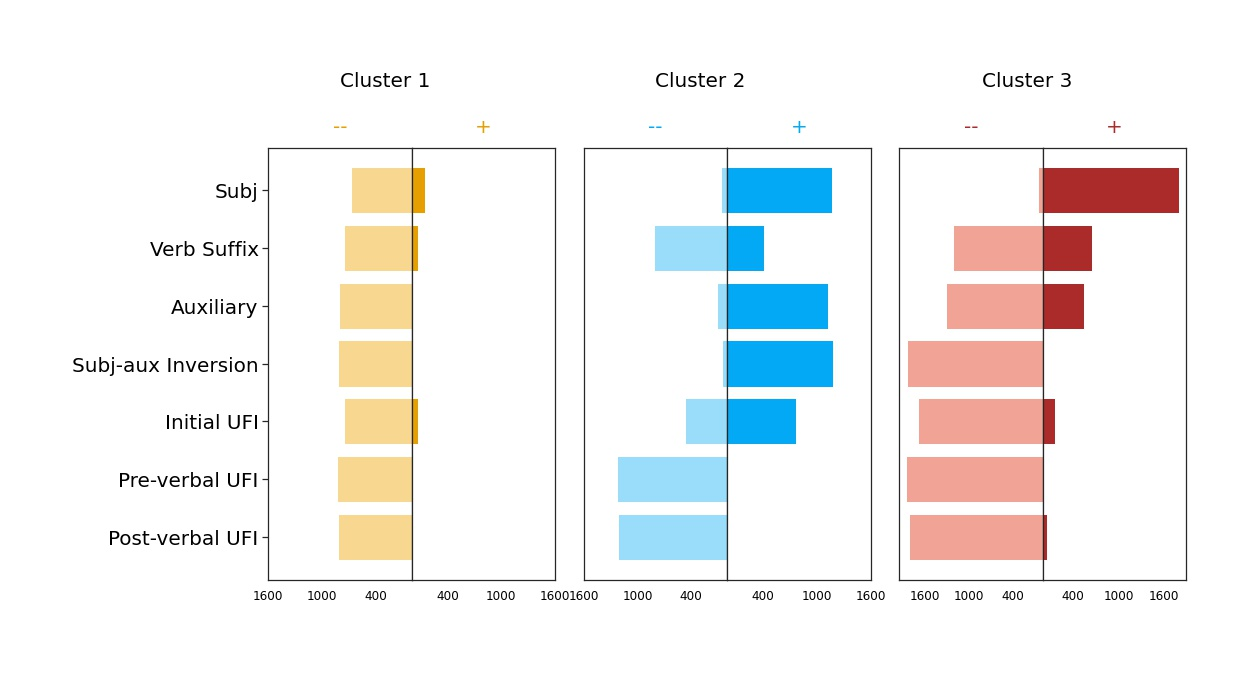
\includegraphics[width=1\textwidth]{figures/target-syncluster-70.jpg}
    \caption{\revise{The morpho-syntactic profile of each cluster in simulations with 70\% noise in speech act information (Cluster 1 $\sim$ Interrogatives, Cluster 2 $\sim$ Imperatives, Cluster 3 $\sim$ Declaratives).}}
    \label{fig:noisy70-syncluster}
\end{figure}

Results from our simulations suggest that morphosyntax is not sufficient to solve the clustering problem, and a small amount of pragmatic information is necessary.

\section{Discussion}
\label{sec:engcl:discussion}

This chapter investigates how 18-month-olds learn to identify the three clause types in English. Our corpus study provides evidence suggesting that the information that children need to solve the clustering and labeling problems for acquiring clause types is present in their input. Parents use clause types systematically, and the three clause types are predominantly mapped to their canonical functions (declaratives to assertions, interrogatives to questions, imperatives to requests/commands) despite the presence of the theoretically expected exceptions to this mapping. The three clause types also show systematically different formal profiles in the input: compared to declaratives, interrogatives are more likely to have auxiliaries, subject-auxiliary inversion, and clause-initial functional items like \twh{}, which are characteristic of [+int] of $C^{0}$ in English; imperatives are more likely to not have subjects or verb suffixes, which is characteristic of [+imp].


I then investigated the extent to which learners need to rely on pragmatic information (i.e., knowing what speech act a given utterance of sentence is conveying), to solve not just labeling, but the clustering itself. I built two Bayesian clustering models simulating a \distlearner{} (\dlearnerabbr{}) and a \praglearner{} (\plearnerabbr{}). I found that morpho-synatctic information is not sufficient for finding the right clause type clustering and a small amount of pragmatic information is necessary, as the \plearnerabbr{} learner outperforms the \dlearnerabbr{} when we ran the two models with the annotated dataset from our corpus study. In addition, a small amount of pragmatics might suffice; even with 80\% noise, the speech act information still helps improve the performance of the model. So even if the speech act information is not perceived veridically for all utterances, learners can still enjoy its benefits.

\subsection{\revise{Implications for learning clause types}}
\revise{With all of the above results, what conclusion can/can't we draw regarding children's learning of clause types? Here I want to discuss the areas where the models are solving an easier problem than children, where the models are probably given a harder problem.  }

\revise{First, our models assume that the learners have \tit{a priori} knowledge regarding the number of clause type categories in their language. While this is a reasonable assumption given the near-universality of declaratives, interrogatives, and imperatives, there are several ways that the actual task that learners have to solve could be more difficult. For one, children might have to figure out the number of clause types in addition to which sentence belongs to which clause type. This additional inference about number might make the learning problem harder for the child. But it is also possible that children start with the assumption that there are three clause types, and gradually expand to include minor clause type categories like exclamatives.  }

\revise{Moreover, I assumed that the learners at this age can perceive a set of morpho-syntactic features that are relevant for clause typing. But this set of features were hand-picked to give the \dlearnerabbr{} model the best chance to succeed; children not be so lucky to have this set picked for them and might need to figure out what are the relevant features for clause typing in addition to figuring out which features go with which clause type cluster. This will no doubt make the learning problem harder. One justification for making this assumption though is that (besides giving the \dlearnerabbr{} the best shot) children might have some knowledge that certain features are clausal features, and some are not. For example, they might know that verb objects might be relevant for learning properties about verbs, but not necessarily relevant for learning the properties of the whole clause. This knowledge might help them pick the relevant morpho-syntactic features for figuring out clause type clusters.
}

\revise{Another area where we could improve the model is how speech act information is accessed by the learner. In our simulations with different noise levels, we replaced a proportion of true speech act labels with random speech act labels. In other words, the models assumed that every utterance you hear is associated with a speech act category; if you are uncertain, you still need to make a guess. But it is very likely that in cases of uncertainty, instead of make a guess, the learner simply tosses out the utterance, so they might not learn from this datapoint. In fact, we adults do this too: sometimes when we can't decide whether our interlocutor is asking a question or making a statement, instead of making a guess right away, we might decide to skip this utterance and wait for more data. Therefore, my next step is to adjust the model to incorporate an internal signal of confidence about speech act perception. This signal could then be used as a filter to help learners only learn from utterances that they are confident about.  }


\revise{One area that the models are given a disadvantage is the absence of prosodic features. We will come back to these features in Chapter~\ref{chap:prosody}.  }

Now that we have established the importance of pragmatics, and that a small amount of pragmatics might suffice, the question then is, how children may get this pragmatic information. How can children infer speech act independently of clause types?  As we have discussed in Chapter~\ref{chap:introduction}, With the innate knowledge of a set of speech act categories and what speech acts do, and a theory of communication, children might have certain expectations about how each speech acts are performed in the input. If these expectations are met, then they can use these cues to infer which utterance is performed with what speech act. But just as our discussion with clause types, behaviors related to speech acts might be absent or misleading. We therefore need to very empirically whether some of these expectations about speech acts can be met. Specifically, is certain prosodic contours and non-linguistic behavior of parents correlate with the use of questions? We will turn to these questions in Chapter~\ref{chap:eng-sp}.



%Our next question is then, what about other languages? As we have discussed in Chapter~\ref{chap:background}, languages differ in the formal features of each clause type, and learners need to discover the correlation from input. The distributional learner for English still have some success with clustering, identifying interrogative clauses. However, maybe the formal features are not as informative in other languages. In the next chapter, we will turn to Mandarin learners, and test the two learners with Mandarin input data. 
